% Options for packages loaded elsewhere
\PassOptionsToPackage{unicode}{hyperref}
\PassOptionsToPackage{hyphens}{url}
\documentclass[
]{book}
\usepackage{xcolor}
\usepackage{amsmath,amssymb}
\setcounter{secnumdepth}{5}
\usepackage{iftex}
\ifPDFTeX
  \usepackage[T1]{fontenc}
  \usepackage[utf8]{inputenc}
  \usepackage{textcomp} % provide euro and other symbols
\else % if luatex or xetex
  \usepackage{unicode-math} % this also loads fontspec
  \defaultfontfeatures{Scale=MatchLowercase}
  \defaultfontfeatures[\rmfamily]{Ligatures=TeX,Scale=1}
\fi
\usepackage{lmodern}
\ifPDFTeX\else
  % xetex/luatex font selection
\fi
% Use upquote if available, for straight quotes in verbatim environments
\IfFileExists{upquote.sty}{\usepackage{upquote}}{}
\IfFileExists{microtype.sty}{% use microtype if available
  \usepackage[]{microtype}
  \UseMicrotypeSet[protrusion]{basicmath} % disable protrusion for tt fonts
}{}
\makeatletter
\@ifundefined{KOMAClassName}{% if non-KOMA class
  \IfFileExists{parskip.sty}{%
    \usepackage{parskip}
  }{% else
    \setlength{\parindent}{0pt}
    \setlength{\parskip}{6pt plus 2pt minus 1pt}}
}{% if KOMA class
  \KOMAoptions{parskip=half}}
\makeatother
\usepackage{color}
\usepackage{fancyvrb}
\newcommand{\VerbBar}{|}
\newcommand{\VERB}{\Verb[commandchars=\\\{\}]}
\DefineVerbatimEnvironment{Highlighting}{Verbatim}{commandchars=\\\{\}}
% Add ',fontsize=\small' for more characters per line
\usepackage{framed}
\definecolor{shadecolor}{RGB}{248,248,248}
\newenvironment{Shaded}{\begin{snugshade}}{\end{snugshade}}
\newcommand{\AlertTok}[1]{\textcolor[rgb]{0.94,0.16,0.16}{#1}}
\newcommand{\AnnotationTok}[1]{\textcolor[rgb]{0.56,0.35,0.01}{\textbf{\textit{#1}}}}
\newcommand{\AttributeTok}[1]{\textcolor[rgb]{0.13,0.29,0.53}{#1}}
\newcommand{\BaseNTok}[1]{\textcolor[rgb]{0.00,0.00,0.81}{#1}}
\newcommand{\BuiltInTok}[1]{#1}
\newcommand{\CharTok}[1]{\textcolor[rgb]{0.31,0.60,0.02}{#1}}
\newcommand{\CommentTok}[1]{\textcolor[rgb]{0.56,0.35,0.01}{\textit{#1}}}
\newcommand{\CommentVarTok}[1]{\textcolor[rgb]{0.56,0.35,0.01}{\textbf{\textit{#1}}}}
\newcommand{\ConstantTok}[1]{\textcolor[rgb]{0.56,0.35,0.01}{#1}}
\newcommand{\ControlFlowTok}[1]{\textcolor[rgb]{0.13,0.29,0.53}{\textbf{#1}}}
\newcommand{\DataTypeTok}[1]{\textcolor[rgb]{0.13,0.29,0.53}{#1}}
\newcommand{\DecValTok}[1]{\textcolor[rgb]{0.00,0.00,0.81}{#1}}
\newcommand{\DocumentationTok}[1]{\textcolor[rgb]{0.56,0.35,0.01}{\textbf{\textit{#1}}}}
\newcommand{\ErrorTok}[1]{\textcolor[rgb]{0.64,0.00,0.00}{\textbf{#1}}}
\newcommand{\ExtensionTok}[1]{#1}
\newcommand{\FloatTok}[1]{\textcolor[rgb]{0.00,0.00,0.81}{#1}}
\newcommand{\FunctionTok}[1]{\textcolor[rgb]{0.13,0.29,0.53}{\textbf{#1}}}
\newcommand{\ImportTok}[1]{#1}
\newcommand{\InformationTok}[1]{\textcolor[rgb]{0.56,0.35,0.01}{\textbf{\textit{#1}}}}
\newcommand{\KeywordTok}[1]{\textcolor[rgb]{0.13,0.29,0.53}{\textbf{#1}}}
\newcommand{\NormalTok}[1]{#1}
\newcommand{\OperatorTok}[1]{\textcolor[rgb]{0.81,0.36,0.00}{\textbf{#1}}}
\newcommand{\OtherTok}[1]{\textcolor[rgb]{0.56,0.35,0.01}{#1}}
\newcommand{\PreprocessorTok}[1]{\textcolor[rgb]{0.56,0.35,0.01}{\textit{#1}}}
\newcommand{\RegionMarkerTok}[1]{#1}
\newcommand{\SpecialCharTok}[1]{\textcolor[rgb]{0.81,0.36,0.00}{\textbf{#1}}}
\newcommand{\SpecialStringTok}[1]{\textcolor[rgb]{0.31,0.60,0.02}{#1}}
\newcommand{\StringTok}[1]{\textcolor[rgb]{0.31,0.60,0.02}{#1}}
\newcommand{\VariableTok}[1]{\textcolor[rgb]{0.00,0.00,0.00}{#1}}
\newcommand{\VerbatimStringTok}[1]{\textcolor[rgb]{0.31,0.60,0.02}{#1}}
\newcommand{\WarningTok}[1]{\textcolor[rgb]{0.56,0.35,0.01}{\textbf{\textit{#1}}}}
\usepackage{longtable,booktabs,array}
\usepackage{calc} % for calculating minipage widths
% Correct order of tables after \paragraph or \subparagraph
\usepackage{etoolbox}
\makeatletter
\patchcmd\longtable{\par}{\if@noskipsec\mbox{}\fi\par}{}{}
\makeatother
% Allow footnotes in longtable head/foot
\IfFileExists{footnotehyper.sty}{\usepackage{footnotehyper}}{\usepackage{footnote}}
\makesavenoteenv{longtable}
\usepackage{graphicx}
\makeatletter
\newsavebox\pandoc@box
\newcommand*\pandocbounded[1]{% scales image to fit in text height/width
  \sbox\pandoc@box{#1}%
  \Gscale@div\@tempa{\textheight}{\dimexpr\ht\pandoc@box+\dp\pandoc@box\relax}%
  \Gscale@div\@tempb{\linewidth}{\wd\pandoc@box}%
  \ifdim\@tempb\p@<\@tempa\p@\let\@tempa\@tempb\fi% select the smaller of both
  \ifdim\@tempa\p@<\p@\scalebox{\@tempa}{\usebox\pandoc@box}%
  \else\usebox{\pandoc@box}%
  \fi%
}
% Set default figure placement to htbp
\def\fps@figure{htbp}
\makeatother
\setlength{\emergencystretch}{3em} % prevent overfull lines
\providecommand{\tightlist}{%
  \setlength{\itemsep}{0pt}\setlength{\parskip}{0pt}}
\usepackage[]{natbib}
\bibliographystyle{plainnat}
\usepackage{booktabs}
\usepackage{bookmark}
\IfFileExists{xurl.sty}{\usepackage{xurl}}{} % add URL line breaks if available
\urlstyle{same}
\hypersetup{
  pdftitle={Week 1: Getting Started with Stata},
  pdfauthor={Samuel Rowe adapted from Acock (2023)},
  hidelinks,
  pdfcreator={LaTeX via pandoc}}

\title{Week 1: Getting Started with Stata}
\author{Samuel Rowe adapted from Acock (2023)}
\date{2026-08-04}

\begin{document}
\maketitle

{
\setcounter{tocdepth}{1}
\tableofcontents
}
\begin{Shaded}
\begin{Highlighting}[]
\NormalTok{bookdown}\SpecialCharTok{::}\FunctionTok{render\_book}\NormalTok{()}
\end{Highlighting}
\end{Shaded}

\chapter*{Overview}\label{overview}
\addcontentsline{toc}{chapter}{Overview}

Topics:

\begin{enumerate}
\def\labelenumi{\arabic{enumi}.}
\tightlist
\item
  Getting Started with Stata
\item
  Entering Data
\item
  Command Line, Do Files, and Results
\end{enumerate}

\chapter{Getting Started}\label{getting-started}

\section{Introduction to Stata}\label{introduction-to-stata}

Stata is a type of \textbf{statistical software package} that can be utilized for data management, data analysis, and statistics. It is similar to other types of statistical software packages compared to R, SAS, or SPSS. It can create reports, regressions, and graphics that can be incorporated into our deliverables.

I have used all of these statistical software packages. While I am a big fan of R, especially with its flexibility, I find that Stata is great for econometric analysis. In my experience Stata stands out in a few ways.

\begin{enumerate}
\def\labelenumi{\arabic{enumi}.}
\tightlist
\item
  Stata is more powerful and flexible than SPSS (IMO)
\item
  Stata's syntax and processing is more streamlined/efficient than SAS (IMO)
\item
  Stata is easier to use than R (IMO)
\end{enumerate}

\section{Get Supporting Material}\label{get-supporting-material}

Before we get started with the Introduction to Stata. I want to make sure everyone is able to download the data.

\begin{Shaded}
\begin{Highlighting}[]
\NormalTok{cd }\StringTok{"/Users/Sam/Desktop/Econ 643/AGIS/"}
\NormalTok{net from https:}\CommentTok{//www.stata{-}press.com/data/agis6r/}
\NormalTok{net }\FunctionTok{get}\NormalTok{ agis6r}
\end{Highlighting}
\end{Shaded}

After we run these commands, we can check to see if the files installed on our local folder

\begin{Shaded}
\begin{Highlighting}[]
\NormalTok{ls}
\end{Highlighting}
\end{Shaded}

\begin{verbatim}
total 19784
-rw-r--r--  1 Sam  staff  5784501 Aug  2 15:14 altrightcombined.dta
-rw-r--r--  1 Sam  staff    37639 Aug  2 15:14 attitude.dta
-rw-r--r--  1 Sam  staff     3715 Aug  2 15:14 c10interaction.dta
-rw-r--r--  1 Sam  staff     3131 Aug  2 15:14 c11barchart.dta
-rw-r--r--  1 Sam  staff     7650 Aug  2 15:14 census.dta
-rw-r--r--  1 Sam  staff      543 Aug  2 15:14 chapter1.do
-rw-r--r--  1 Sam  staff     4453 Aug  2 15:14 chapter10.do
-rw-r--r--  1 Sam  staff     2982 Aug  2 15:14 chapter11.do
-rw-r--r--  1 Sam  staff     3194 Aug  2 15:14 chapter12.do
-rw-r--r--  1 Sam  staff     1016 Aug  2 15:14 chapter13.do
-rw-r--r--  1 Sam  staff    92863 Aug  2 15:14 chapter14_missing.dta
-rw-r--r--  1 Sam  staff     1604 Aug  2 15:14 chapter14.do
-rw-r--r--  1 Sam  staff     3124 Aug  2 15:14 chapter15.do
-rw-r--r--  1 Sam  staff      786 Aug  2 15:14 chapter16.do
-rw-r--r--  1 Sam  staff      363 Aug  2 15:14 chapter2.do
-rw-r--r--  1 Sam  staff     2688 Aug  2 15:14 chapter3.do
-rw-r--r--  1 Sam  staff      578 Aug  2 15:14 chapter4.do
-rw-r--r--  1 Sam  staff     1411 Aug  2 15:14 chapter5.do
-rw-r--r--  1 Sam  staff   267702 Aug  2 15:14 chapter6_aspirin.dta
-rw-r--r--  1 Sam  staff     1096 Aug  2 15:14 chapter6.do
-rw-r--r--  1 Sam  staff     2772 Aug  2 15:14 chapter7.do
-rw-r--r--  1 Sam  staff     2272 Aug  2 15:14 chapter8.do
-rw-r--r--  1 Sam  staff     2854 Aug  2 15:14 chapter9.do
-rw-r--r--  1 Sam  staff     1845 Aug  2 15:14 chores.dta
-rw-r--r--  1 Sam  staff    65280 Aug  2 15:14 descriptive_gss.dta
-rw-r--r--  1 Sam  staff     1875 Aug  2 15:14 divorce.dta
-rw-r--r--  1 Sam  staff     1875 Aug  2 15:14 environ.dta
-rw-r--r--  1 Sam  staff     6682 Aug  2 15:14 firstsurvey_chapter4.dta
-rw-r--r--  1 Sam  staff     7720 Aug  2 15:14 firstsurvey.dta
-rw-r--r--  1 Sam  staff    17530 Aug  2 15:14 flourishing_bmi.dta
-rw-r--r--  1 Sam  staff   196040 Aug  2 15:14 gss2002_and_2006_chapter12.dta
-rw-r--r--  1 Sam  staff    71890 Aug  2 15:14 gss2002_chapter10.dta
-rw-r--r--  1 Sam  staff    70433 Aug  2 15:14 gss2002_chapter11.dta
-rw-r--r--  1 Sam  staff    54891 Aug  2 15:14 gss2002_chapter6.dta
-rw-r--r--  1 Sam  staff    36806 Aug  2 15:14 gss2002_chapter7.dta
-rw-r--r--  1 Sam  staff    48506 Aug  2 15:14 gss2002_chapter7b.dta
-rw-r--r--  1 Sam  staff    47388 Aug  2 15:14 gss2002_chapter8.dta
-rw-r--r--  1 Sam  staff    36438 Aug  2 15:14 gss2002_chapter9.dta
-rw-r--r--  1 Sam  staff   123729 Aug  2 15:14 gss2006_chapter12_selected.dta
-rw-r--r--  1 Sam  staff   254116 Aug  2 15:14 gss2006_chapter12.dta
-rw-r--r--  1 Sam  staff    19937 Aug  2 15:14 gss2006_chapter6_10percent.dta
-rw-r--r--  1 Sam  staff    84882 Aug  2 15:14 gss2006_chapter6.dta
-rw-r--r--  1 Sam  staff    11282 Aug  2 15:14 gss2006_chapter8_selected.dta
-rw-r--r--  1 Sam  staff   143277 Aug  2 15:14 gss2006_chapter8.dta
-rw-r--r--  1 Sam  staff    73780 Aug  2 15:14 gss2006_chapter9_2way.dta
-rw-r--r--  1 Sam  staff    63099 Aug  2 15:14 gss2006_chapter9.dta
-rw-r--r--  1 Sam  staff    64584 Aug  2 15:14 gss2016_chapter12.dta
-rw-r--r--  1 Sam  staff     4563 Aug  2 15:14 highjump.dta
-rw-r--r--  1 Sam  staff     1974 Aug  2 15:14 intraclass.dta
-rw-r--r--  1 Sam  staff    23745 Aug  2 15:14 irt_exercises.dta
-rw-r--r--  1 Sam  staff     2102 Aug  2 15:14 kappa1.dta
-rw-r--r--  1 Sam  staff    13444 Aug  2 15:14 kuder-richardson.dta
-rw-r--r--  1 Sam  staff     1915 Aug  2 15:14 long.dta
-rw-r--r--  1 Sam  staff   108658 Aug  2 15:14 longitudinal_exercise.dta
-rw-r--r--  1 Sam  staff    63905 Aug  2 15:14 longitudinal_mixed.dta
-rw-r--r--  1 Sam  staff   615085 Aug  2 15:14 nlsy97_chapter11.dta
-rw-r--r--  1 Sam  staff    58476 Aug  2 15:14 nlsy97_chapter7.dta
-rw-r--r--  1 Sam  staff   541933 Aug  2 15:14 nlsy97_selected_variables.dta
-rw-r--r--  1 Sam  staff   166013 Aug  2 15:14 ops2004.dta
-rw-r--r--  1 Sam  staff     4663 Aug  2 15:14 partyid.dta
-rw-r--r--  1 Sam  staff     7809 Aug  2 15:14 relate.cdb
-rw-r--r--  1 Sam  staff   225118 Aug  2 15:14 relate.dct
-rw-r--r--  1 Sam  staff   402891 Aug  2 15:14 relate.dta
-rw-r--r--  1 Sam  staff     1855 Aug  2 15:14 retest.dta
-rw-r--r--  1 Sam  staff     5955 Aug  2 15:14 severity.dta
-rw-r--r--  1 Sam  staff     3165 Aug  2 15:14 spearman.dta
-rw-r--r--  1 Sam  staff     1875 Aug  2 15:14 wide.dta
-rw-r--r--  1 Sam  staff     4529 Aug  2 15:14 wide9.dta
\end{verbatim}

We will be utilizing these data and do files throughout the course.

Also, I will be working with Stata 19, but it is okay if you are working with Stata 17 or Stata 18.

\section{Stata Screen}\label{stata-screen}

For those who have never used Stata before. Let's navigate the screen.

\begin{figure}
\centering
\pandocbounded{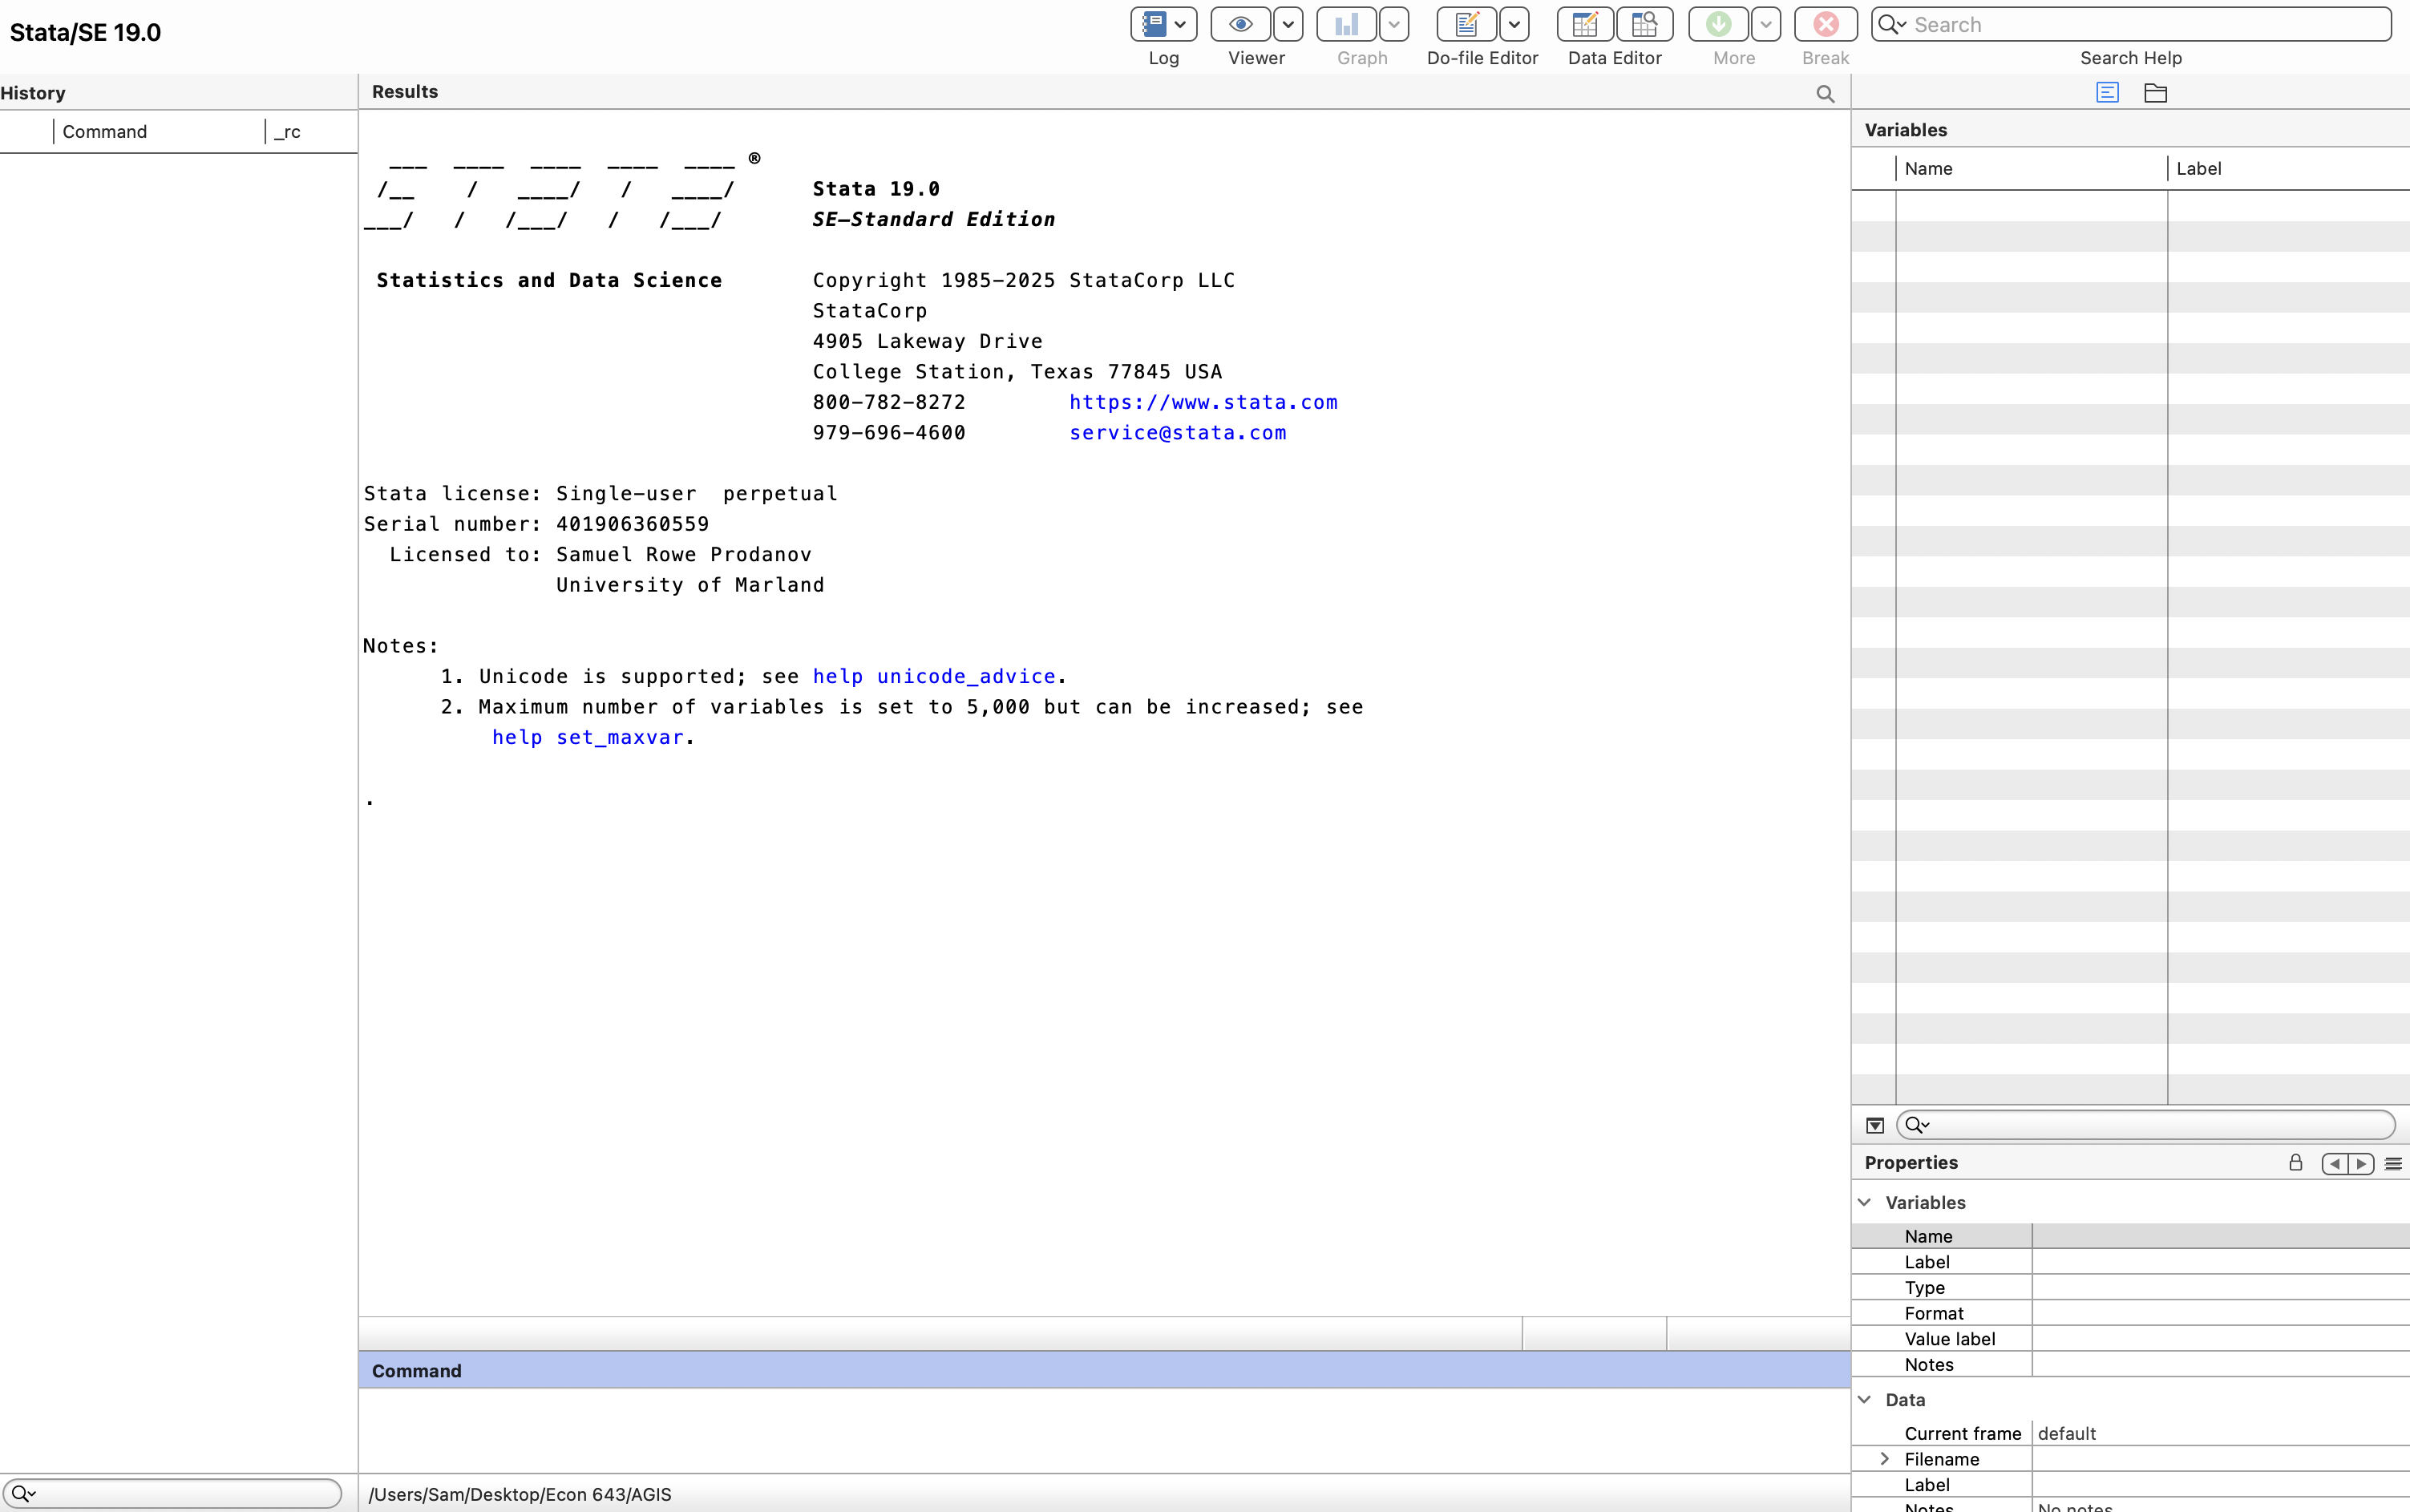
\includegraphics[keepaspectratio,alt={Stata Window}]{week1_empty.png}}
\caption{Stata Window}
\end{figure}

The \textbf{output} or \textbf{results} window is the middle of the screen and provides the largest section in Stata.

Below the \textbf{output} window is the \textbf{command line} window. Here you can enter ad hoc commands. I personally find these very helpful with data exploration using the \emph{tabulate} or \emph{sum} commands.

On the left-most side is the \textbf{command history} window. This will show prior commands that you have run through the \textbf{command line}. This is helpful if you need to copy something over to a \textbf{do file} or run a prior command.

In the upper right, we have the \textbf{variable} window. This window provides information about the variables in your dataset. Once you select a variable in the \textbf{variable} window, information about the variable appears in the lower-right window or \textbf{variable property} window.

Stata's Toolbar provides helpful quick clicks for Stata's Tools

\begin{figure}
\centering
\pandocbounded{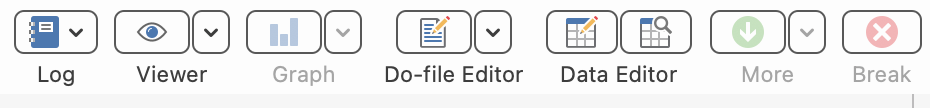
\includegraphics[keepaspectratio,alt={Stata toolbar for OSX}]{week1_ribbon.png}}
\caption{Stata toolbar for OSX}
\end{figure}

The most important button is going to be the \textbf{Do-File Editor} button. This is where you do the majority of your work in Stata. The table with the magnifing glass is another important button for a quick click to the \textbf{Browser} window.

\section{Our First Dataset}\label{our-first-dataset}

\textbf{Please note that we will be working through the Do-File editor. We will not be using the point-and-click method}

Let's go ahead and use a dataset in memory. We will use the command \emph{sysuse} with the option clear.

\begin{Shaded}
\begin{Highlighting}[]
\KeywordTok{sysuse}\NormalTok{ cancer, }\KeywordTok{clear}
\end{Highlighting}
\end{Shaded}

\begin{figure}
\centering
\pandocbounded{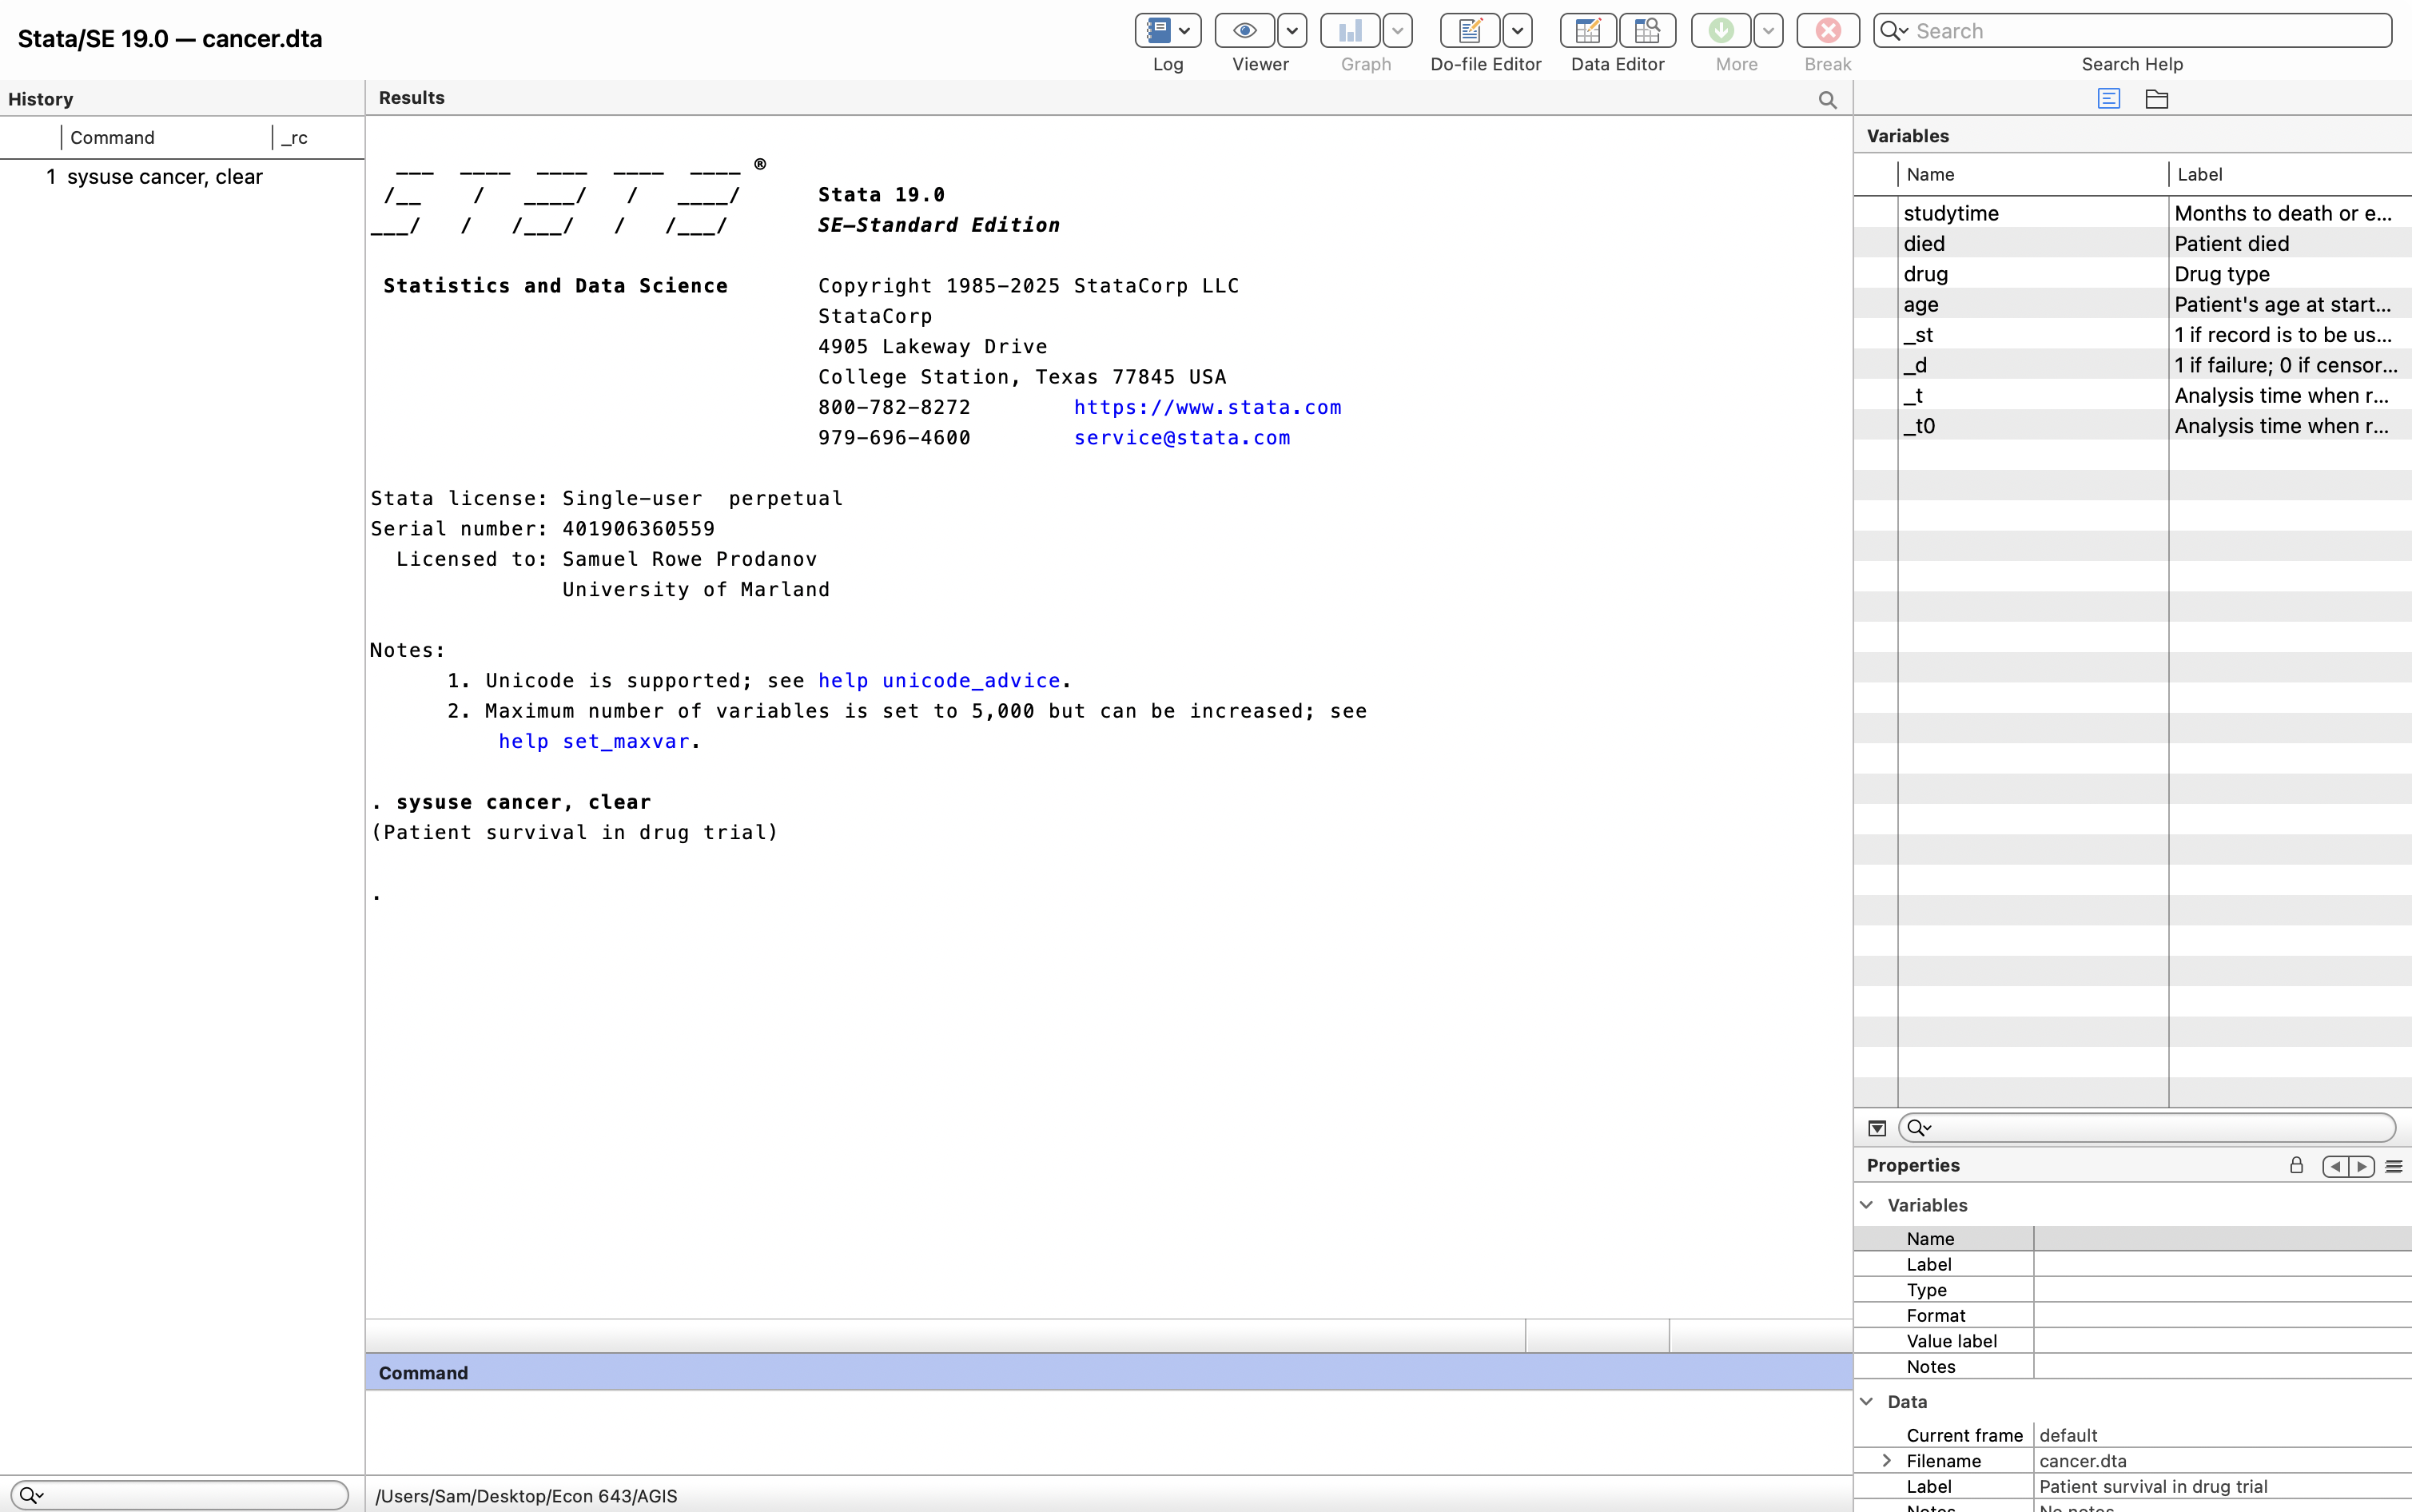
\includegraphics[keepaspectratio,alt={Stata Window with Data Loaded}]{week1_sysuse.png}}
\caption{Stata Window with Data Loaded}
\end{figure}

Now we have loaded a dataset into Stata, we can see that our windows hhve changed. Our results window says

. sysuse cancer, clear
(Patient survival in drug trial)

Our \textbf{Command History} window shows are last command. Our variables in the memory are shown in the \textbf{Variable} window.

\section{Run commands}\label{run-commands}

\subsection{describe}\label{describe}

Next let's run some commands to do some small analyses. Let's look at the data with the \emph{describe} command.

\begin{Shaded}
\begin{Highlighting}[]
\KeywordTok{describe}
\end{Highlighting}
\end{Shaded}

\begin{verbatim}
Contains data from /Applications/Stata/ado/base/c/cancer.dta
 Observations:            48                  Patient survival in drug trial
    Variables:             8                  3 Mar 2024 16:09
----------------------------------------------------------------------------------
Variable      Storage   Display    Value
    name         type    format    label      Variable label
----------------------------------------------------------------------------------
studytime       byte    %8.0g                 Months to death or end of exp.
died            byte    %8.0g      diedlbl    Patient died
drug            byte    %8.0g      type       Drug type
age             byte    %8.0g                 Patient's age at start of exp.
_st             byte    %8.0g                 1 if record is to be used; 0
                                                otherwise
_d              byte    %8.0g                 1 if failure; 0 if censored
_t              byte    %10.0g                Analysis time when record ends
_t0             byte    %10.0g                Analysis time when record begins
----------------------------------------------------------------------------------
Sorted by: 
\end{verbatim}

The \emph{describe} command gives us an overview of the dataset. It provides the variable name, storage type, display format, value label, and variable label. We can see that all of our data are numeric and have variable labels to describe the variable, but only two variables have labels for the values.

\subsection{summarize}\label{summarize}

Next, we can run basic descriptive statistics for all of our variables with the \emph{summarize} or \emph{sum} command.

\begin{Shaded}
\begin{Highlighting}[]
\KeywordTok{summarize}
\end{Highlighting}
\end{Shaded}

\begin{verbatim}
    Variable |        Obs        Mean    Std. dev.       Min        Max
-------------+---------------------------------------------------------
   studytime |         48        15.5    10.25629          1         39
        died |         48    .6458333    .4833211          0          1
        drug |         48       1.875    .8410986          1          3
         age |         48      55.875    5.659205         47         67
         _st |         48           1           0          1          1
-------------+---------------------------------------------------------
          _d |         48    .6458333    .4833211          0          1
          _t |         48        15.5    10.25629          1         39
         _t0 |         48           0           0          0          0
\end{verbatim}

Our basic descriptive statistics show that the average age is 55.9 years old with a standard deviation of 5.7. Our maximum age is 67 and the minimum age is 47.

\subsection{histogram}\label{histogram}

Next we can graph the distribution of our \emph{age} variable. AGIS shows how to create a histogram with the point and click, but we are going straight to syntax. No point in delaying the inevitable.

\begin{Shaded}
\begin{Highlighting}[]
\KeywordTok{histogram}\NormalTok{ age}
\end{Highlighting}
\end{Shaded}

\begin{verbatim}
(bin=6, start=47, width=3.3333333)
\end{verbatim}

\begin{figure}
\centering
\pandocbounded{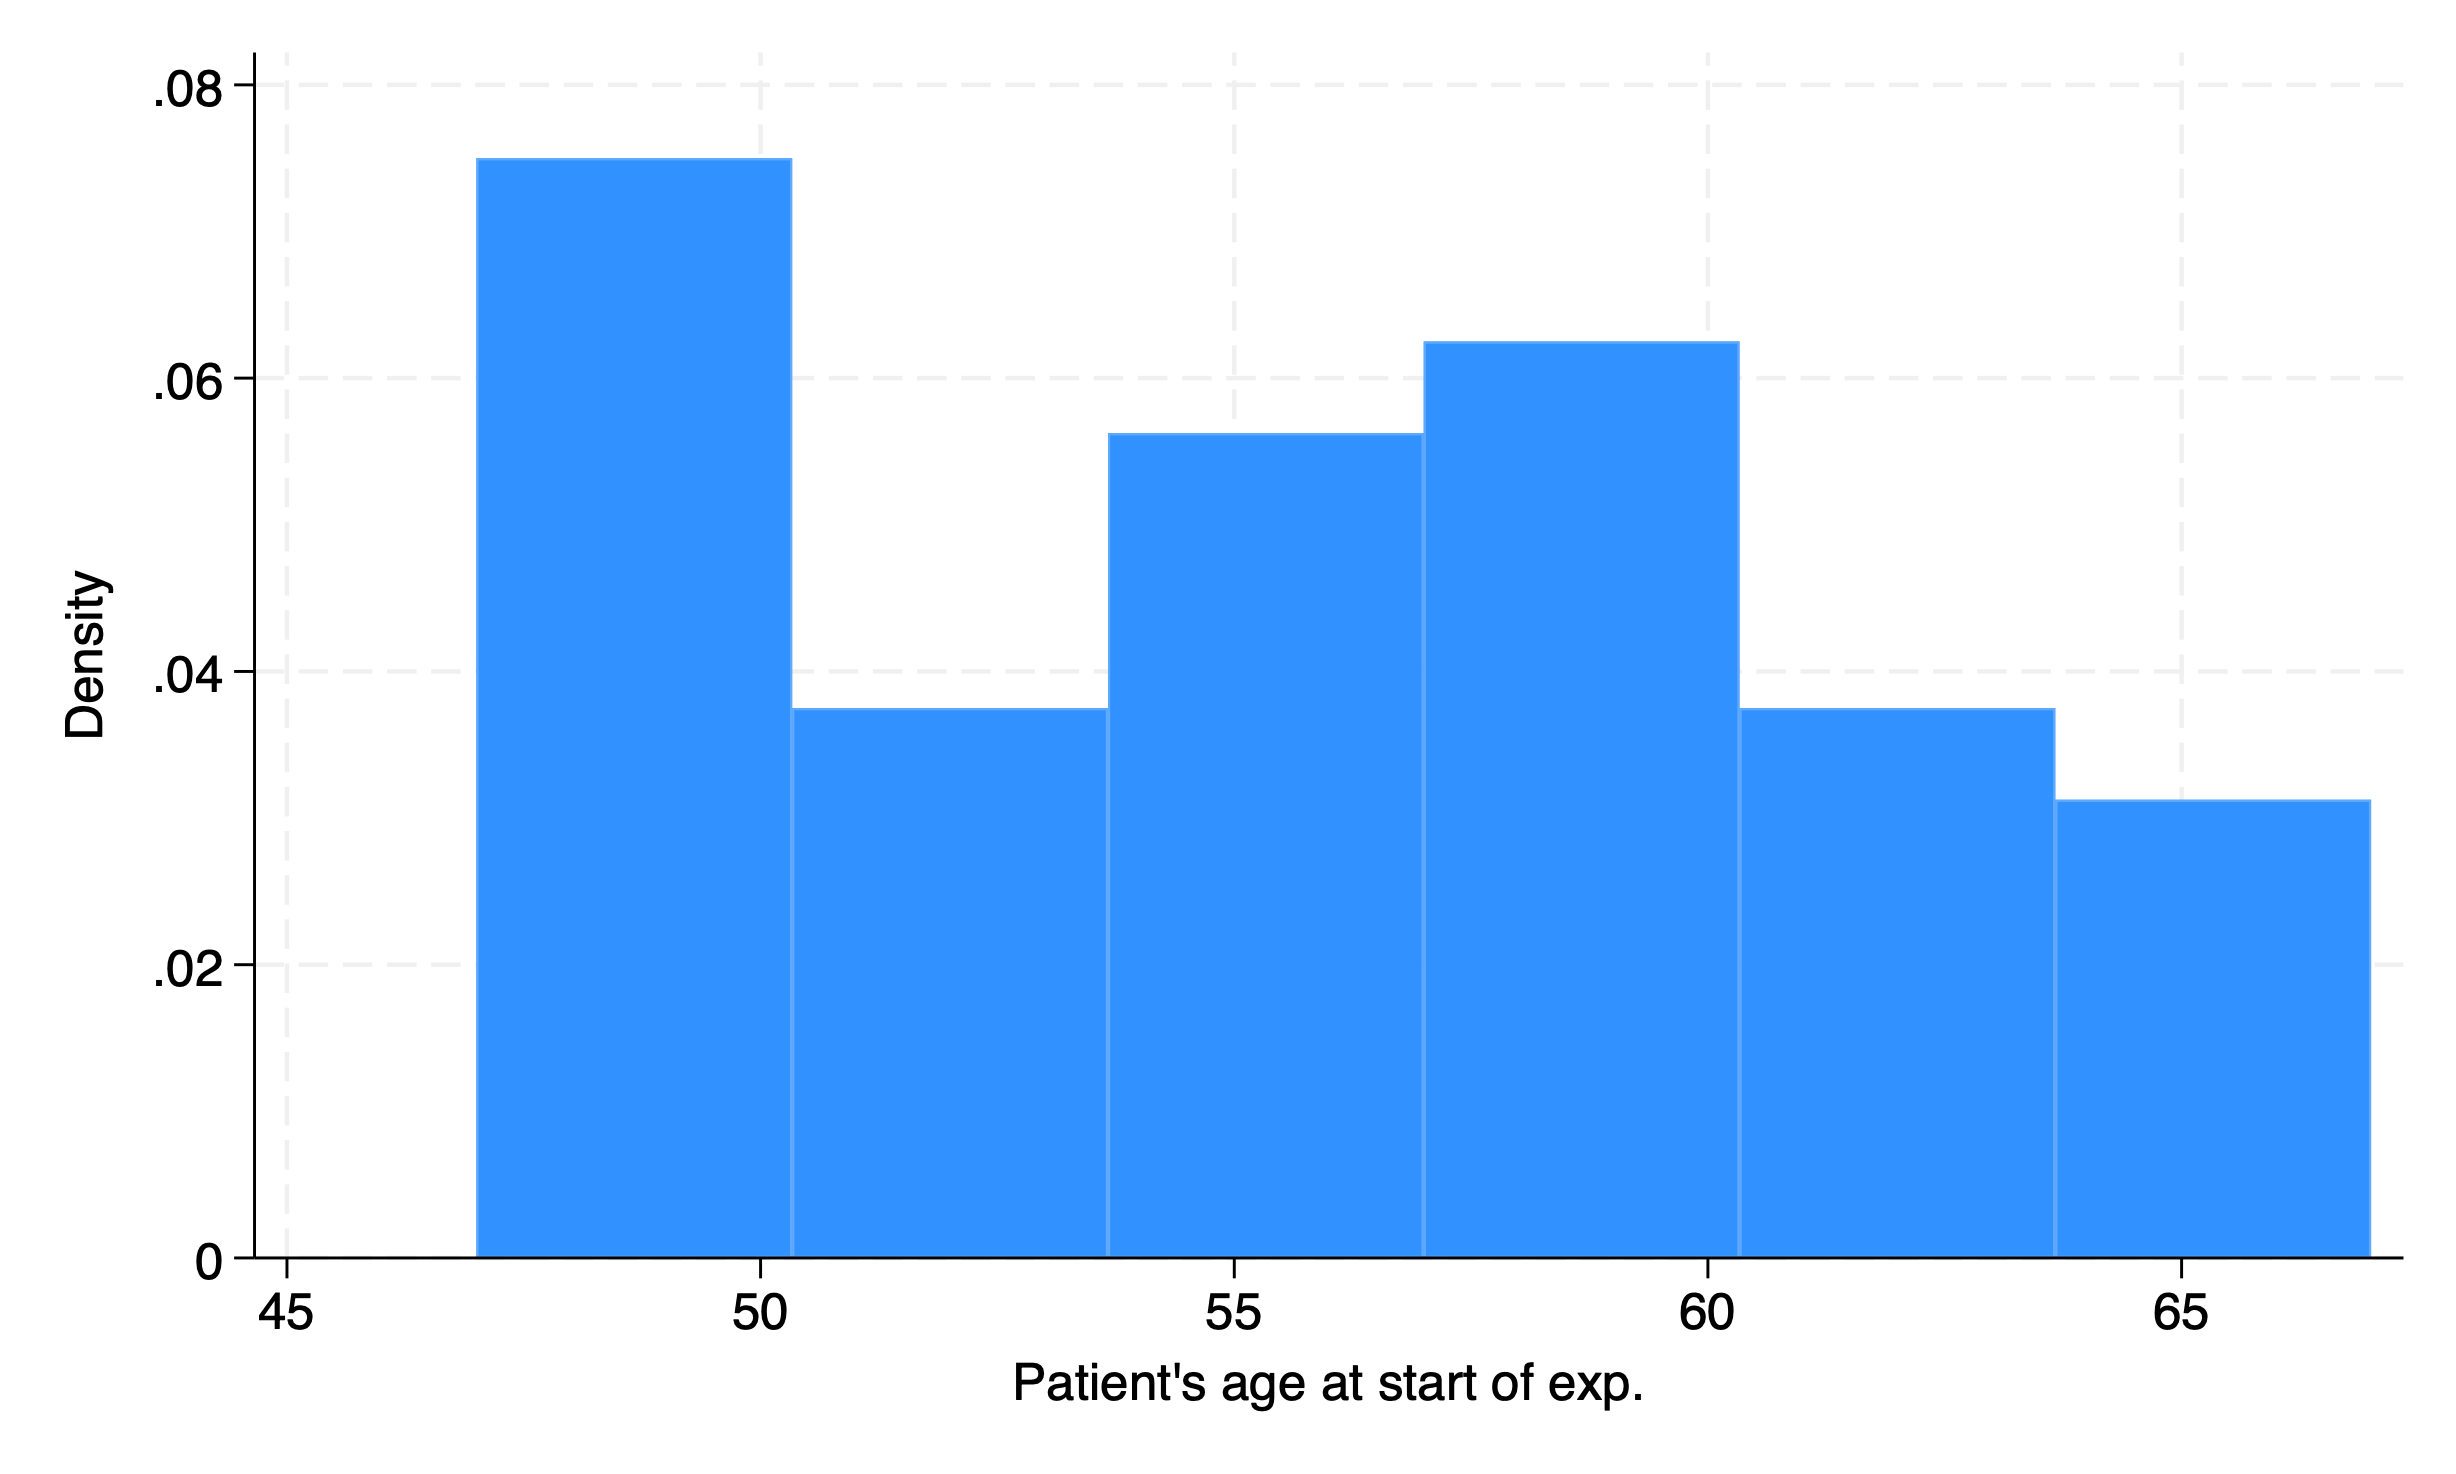
\includegraphics[keepaspectratio,alt={Our first histogram}]{week1_histogram.png}}
\caption{Our first histogram}
\end{figure}

We can format the histogram with options. We can edit the bins and the width of the histogram with the \emph{bin()} option or \emph{width()} options. Options are established after the \textbf{,} in a command. We will also start at age 45 with the \emph{start} option and increment by 2.5 with \emph{width(2.5}. We can also edit the title with the \emph{title()} option and cite the source of the data with the \emph{caption()} option.

\begin{Shaded}
\begin{Highlighting}[]
\KeywordTok{histogram}\NormalTok{ age, }\BaseNTok{title}\NormalTok{(}\StringTok{"Age distribution of participants in cancer study"}\NormalTok{) }\BaseNTok{caption}\NormalTok{(}\StringTok{"Cancer Dataset"}\NormalTok{) }\KeywordTok{width}\NormalTok{(2.5) }\BaseNTok{start}\NormalTok{(45)}
\end{Highlighting}
\end{Shaded}

\begin{verbatim}
(bin=6, start=47, width=3.3333333)
\end{verbatim}

\begin{figure}
\centering
\pandocbounded{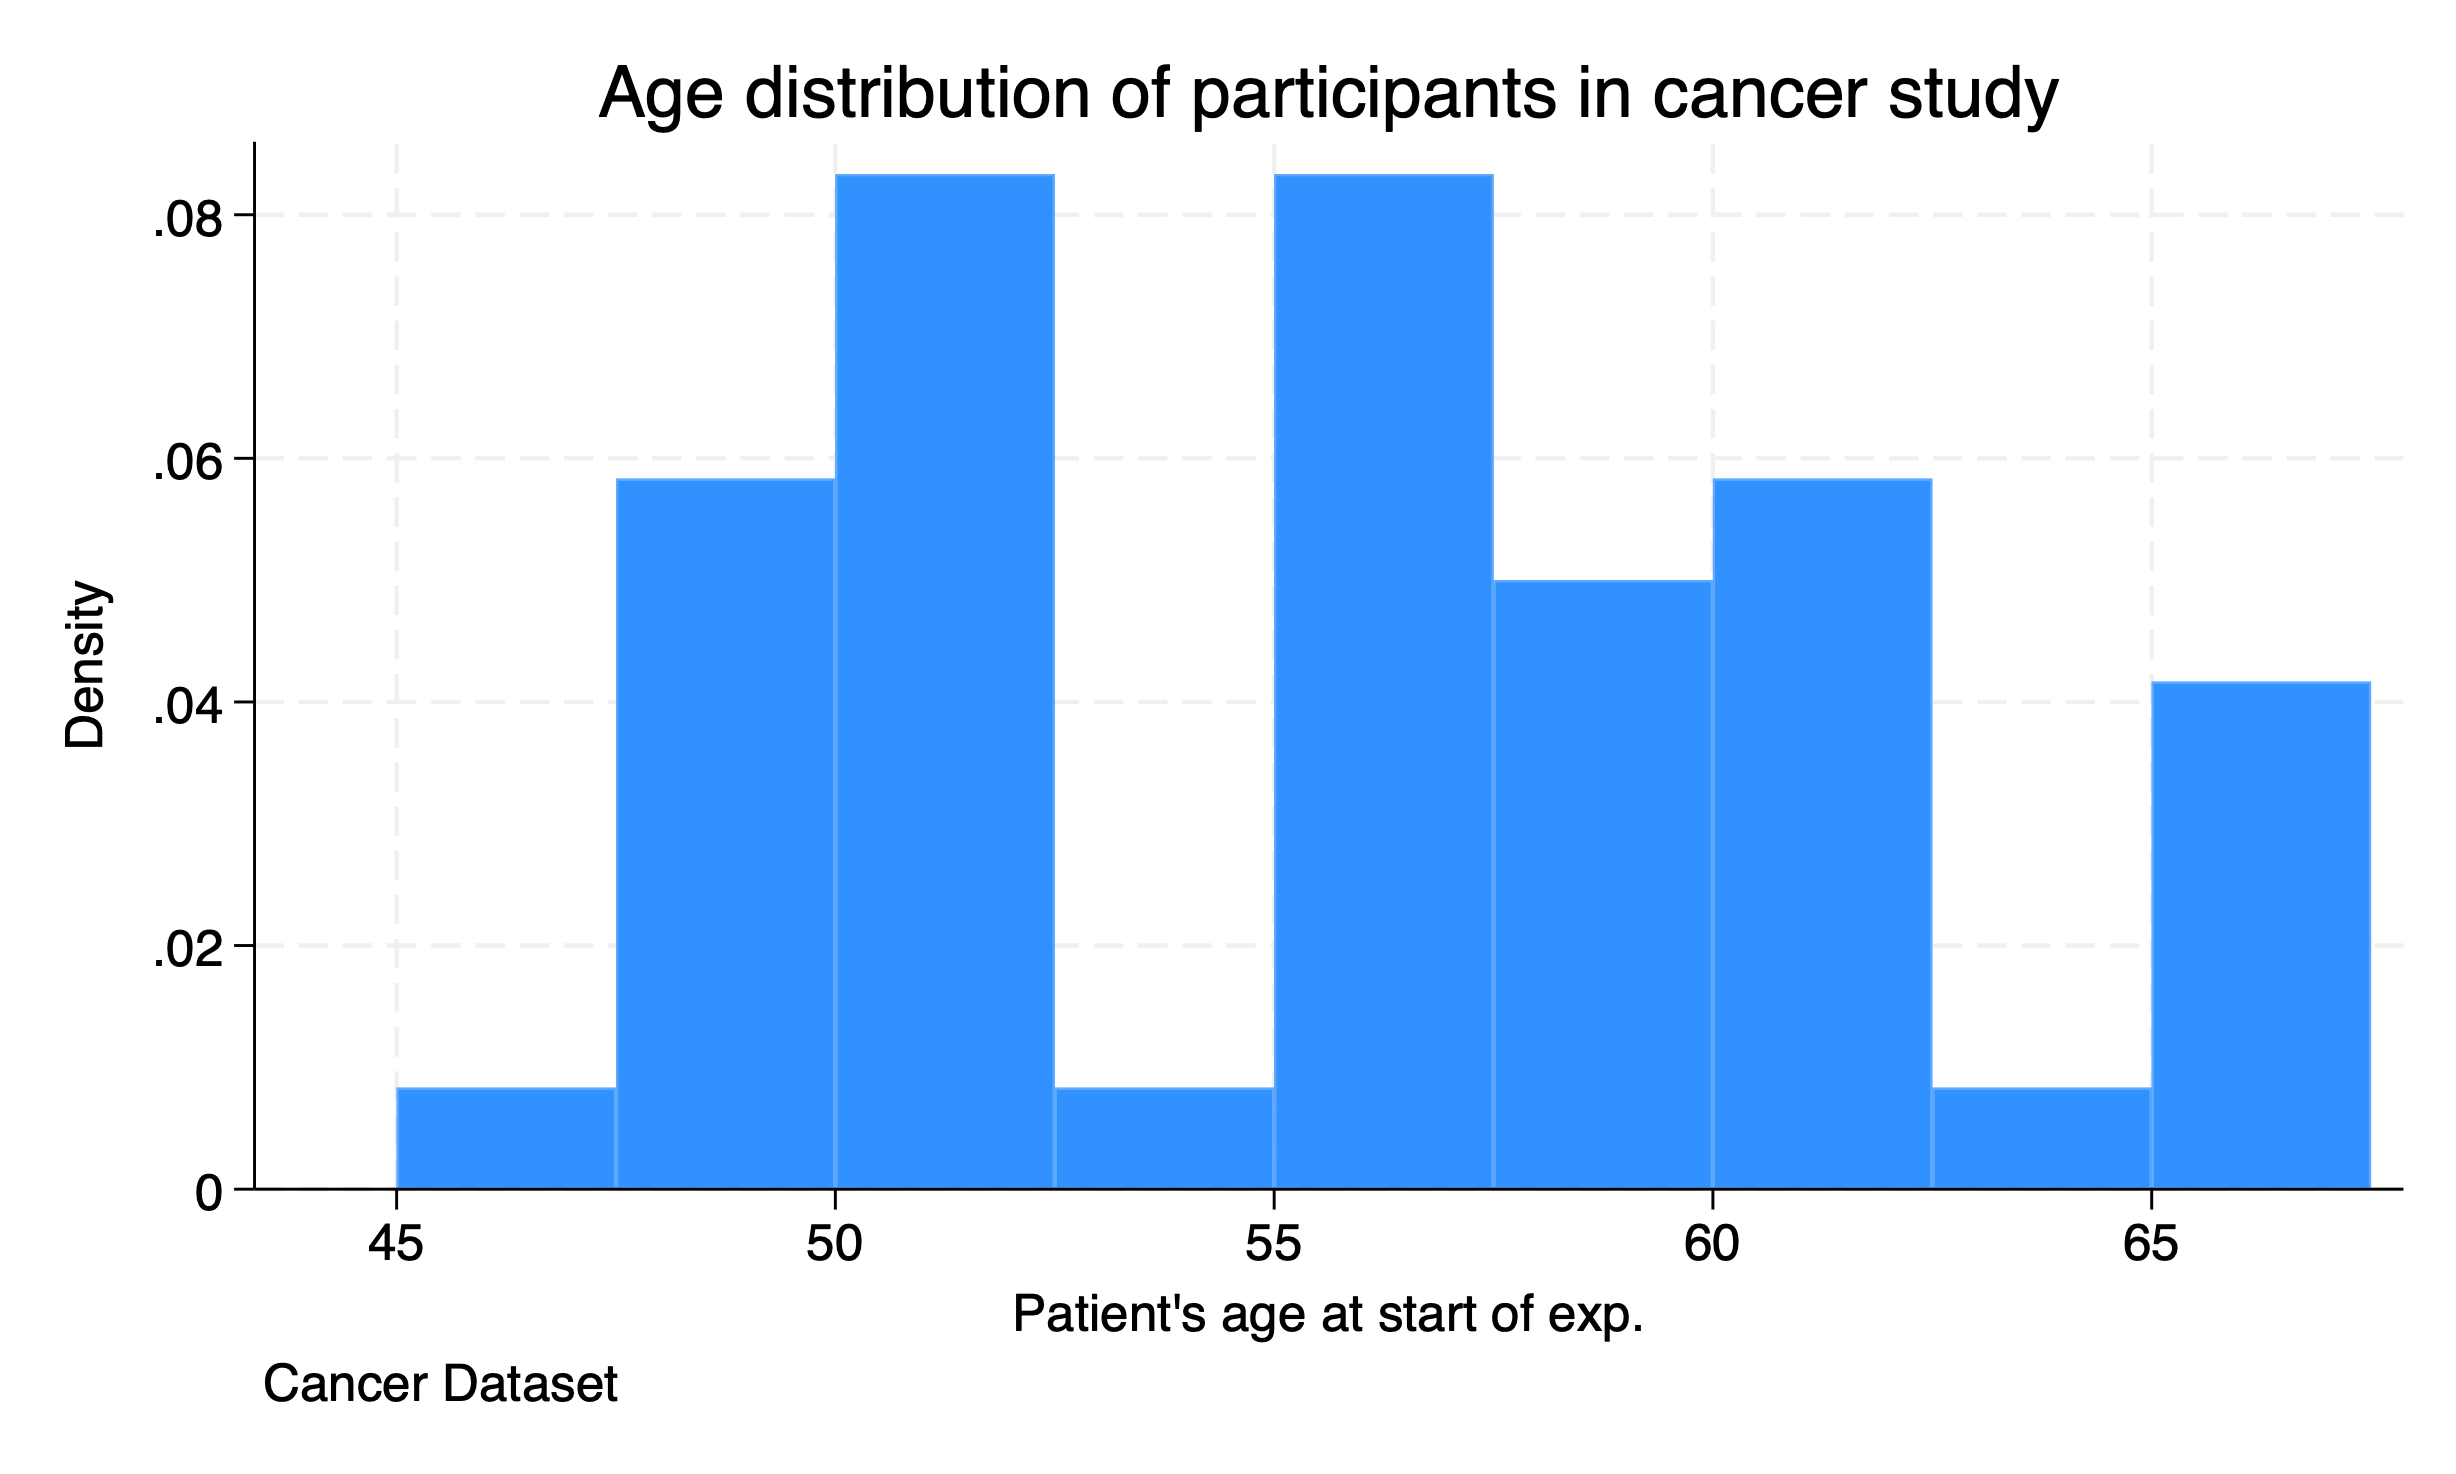
\includegraphics[keepaspectratio,alt={Formatted Histogram}]{week1_histogram_format.png}}
\caption{Formatted Histogram}
\end{figure}

We can see the number of bins has increased and the width of the bins is 2.5 years. We have also added a title and a source of the data.

\section{Help and Search}\label{help-and-search}

Before we get started, I wanted to talk about two helpful commands.

\begin{Shaded}
\begin{Highlighting}[]
\KeywordTok{help} \KeywordTok{tabulate}
\KeywordTok{search} \KeywordTok{tabulate}
\end{Highlighting}
\end{Shaded}

The \emph{help} command displays help information about the specified command or topic, while the \emph{search} command search Stata documentation and other resources. These can be utilized to gather additional information about commands or topics.

\chapter{Entering Data}\label{entering-data}

Before we begin this section, I recommend not working directly in Stata's data editor. This is a personal preference, and you are more than welcome to work directly in the data editor. I generally recommend working in a spreadsheet software and importing the data into Stata. However, we will cover some basics.

If you need to edit data, I recommand using the \emph{replace} command which we will cover later.

\textbf{Please note that if you need to edit data, do not do an ad-hoc edits. Import raw data and use syntax to be transparent!}

\section{ETL}\label{etl}

We will use using an ``ETL'' philosophy. This acronym stands for ``Extract'', ``Transform'', ``Load''. We will ``Extract'' data from its source, so external audience can see the raw data. We will use the \emph{use} or \emph{import using} commands to extract our from our source data. We will cover more on the \emph{import} command when we get to Mitchell (2020).

Next, we need to ``Transform'' the data. We will be using the \emph{generate} and \emph{replace} command to show external users how we made edits. Data transformations in source data can be opaque. We want transparency!

Finally, we will ``Load'' the data. What we are doing here is exporting our data analyses and graphs into our final product, such as presentations and articles. Stata has a variety of methods to create data table that can be used in Word or LaTex.

\section{The Data Editor}\label{the-data-editor}

If we want to manually enter data into stata, \textbf{which I do not recommend}, we can start Stata's data editor. One way is to use the quick click on the toolbar. This is the icon with the table and the pencil.

\begin{figure}
\centering
\pandocbounded{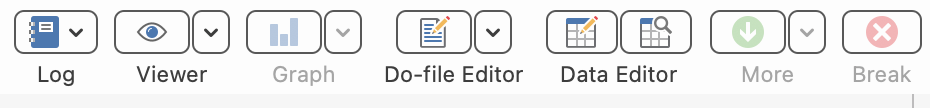
\includegraphics[keepaspectratio,alt={Data Editor in the Toolbar}]{week1_ribbon.png}}
\caption{Data Editor in the Toolbar}
\end{figure}

We can also launch the data editor by typing \emph{edit} into the command line.

\begin{Shaded}
\begin{Highlighting}[]
\NormalTok{edit}
\end{Highlighting}
\end{Shaded}

\begin{figure}
\centering
\pandocbounded{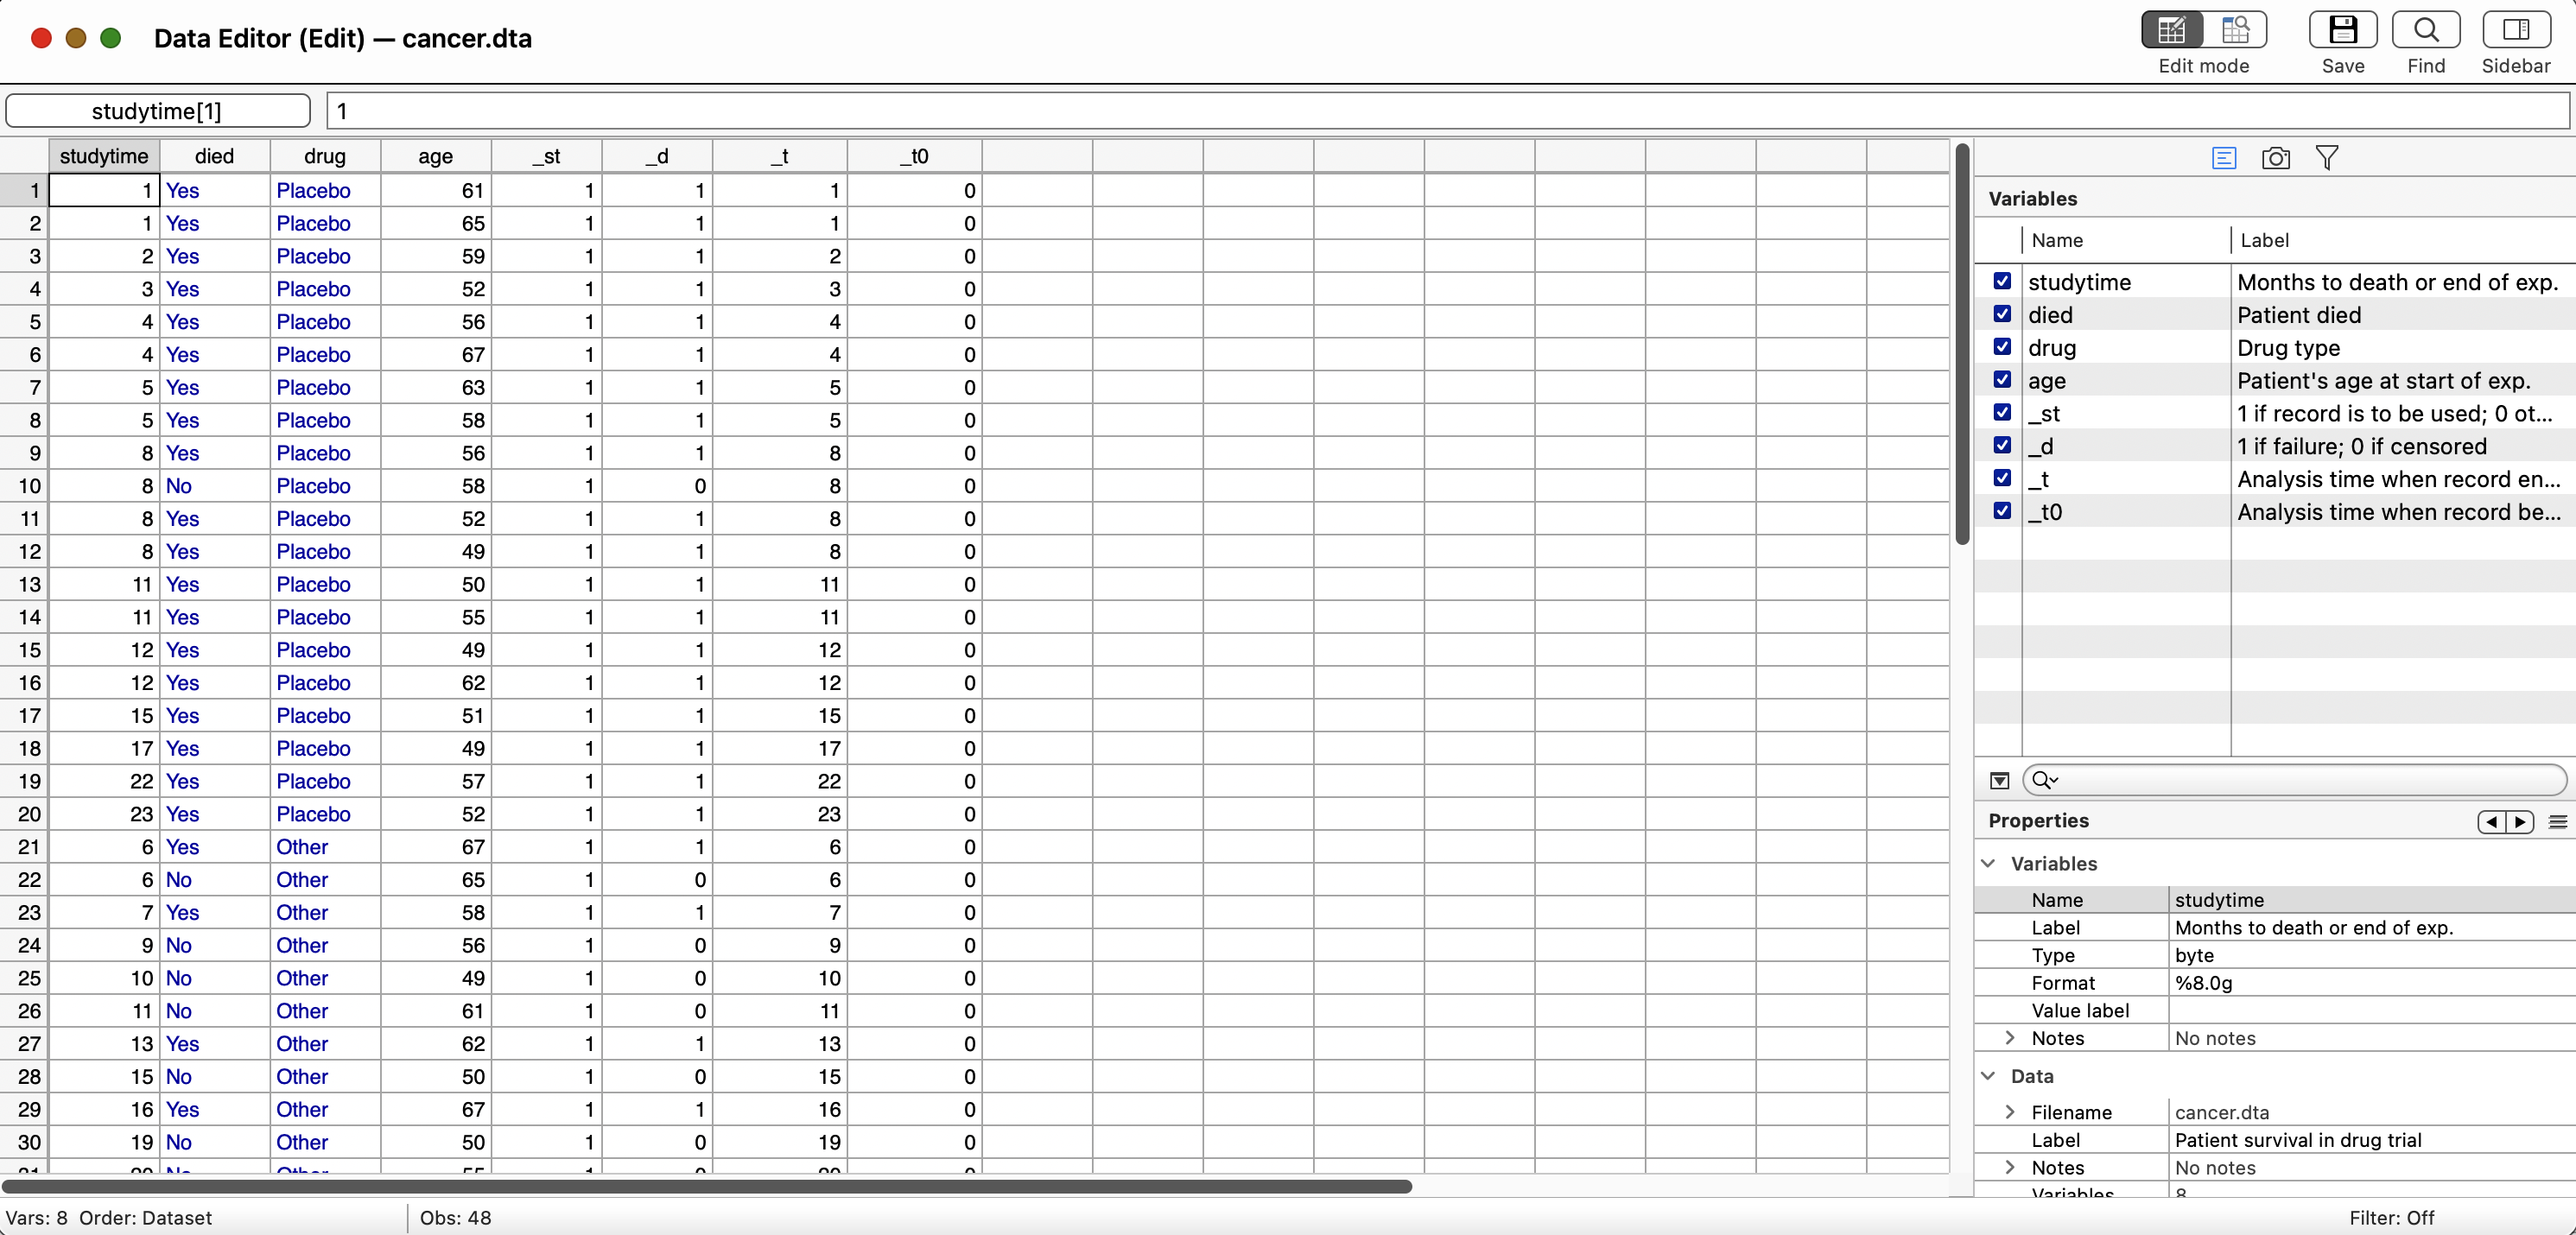
\includegraphics[keepaspectratio,alt={Data Editor}]{week1_editor.png}}
\caption{Data Editor}
\end{figure}

I will not delve into this chapter any farther, since we will use syntax to create, edit, or delete variables. This includes labeling our data. \textbf{Use syntax!}

\chapter{Commands, Do Files, and Results}\label{commands-do-files-and-results}

I don't spend much time on Data Editor, since we should be doing data transformations within our reproducible syntax in our do files. This will be our focus moving forward.

Why use do files? My two main points are the following:
1. Efficiency
2. Transparency

\textbf{Efficiency:} Your future time required to do routine tasks drops immensely once your syntax works. Not only can it reduce time for a routine task, you can take snippits of your syntax for other do files. No point in reinventing the wheel! Point and click may be faster up front, but on routine tasks point-and-clicks get left in the dust compared to syntax.

\textbf{Transparency:} You can provide evidence of your work. An independent person can take the source data independency, and apply your syntax to see if they get similar results. Not only that, they can check for any shenanigans within the syntax. You will see data replication packages in journals of the \emph{American Economic Association}.

\section{Commands}\label{commands}

Before we start working with do files, we should have a base repository of commands, so we can work with data. We will cover other commands, such as \emph{ttest}, \emph{anova}, and \emph{regress} a bit later.

\begin{tabular}{l|l}
\hline
Variables & Description\\
\hline
use & Put a Stata .dta file into Stata's memory\\
\hline
sysuse & Put a shipped or build-in data file into Stata's memory\\
\hline
import & Put a non-Stata file, such as .xslx, into Stata's memory\\
\hline
cd & Change working directory\\
\hline
list & List of the values of variables\\
\hline
summarize & Summary statistics\\
\hline
describe & Describe the data in memory or in file\\
\hline
codebook & Describe the data contents\\
\hline
tabulate & Tables of frequences\\
\hline
generate & Create a variable\\
\hline
replace & Change contents of a variable\\
\hline
egen & Extensions to generate\\
\hline
graph & The graph command\\
\hline
histogram & Creates a histogram\\
\hline
save & Saves a file to designated folder\\
\hline
missing & Is missing\\
\hline
\end{tabular}

These commands will be workhorses for you, so it is good to begin working with them now.

\begin{Shaded}
\begin{Highlighting}[]
\KeywordTok{sysuse}\NormalTok{ Mroz, }\KeywordTok{clear}
\KeywordTok{summarize}\NormalTok{ lwg, }\KeywordTok{detail} 
\end{Highlighting}
\end{Shaded}

\begin{verbatim}
      Log wage rate. Actual wage, or for lfp=0 imputed
               by regressing lwg on other vars
-------------------------------------------------------------
      Percentiles      Smallest
 1%    -.6931472      -2.054124
 5%     .2066842      -1.822531
10%     .4953217      -1.766441       Obs                 753
25%     .8180865      -1.543298       Sum of wgt.         753

50%     1.068403                      Mean           1.097115
                        Largest       Std. dev.      .5875564
75%     1.399717       3.113515
90%     1.760261       3.155581       Variance       .3452226
95%     2.083896       3.218876       Skewness      -.3992074
99%     2.733368       3.218876       Kurtosis       7.040145
\end{verbatim}

We can dig deeper into the command by looking up the options of these command. We can look up the options for the \emph{summarize} command with the following:

\begin{Shaded}
\begin{Highlighting}[]
\KeywordTok{help} \KeywordTok{summarize}
\end{Highlighting}
\end{Shaded}

\section{Qualifiers}\label{qualifiers}

We may want to qualifers for conditional commands. We may want to look at subsets when analzying data or apply a command under certain conditions. Stata's list of qualifiers is the following:

\begin{tabular}{l|l}
\hline
RelationalOperators & Description\\
\hline
== & is or is equal to\\
\hline
!= & is not or is not equal to\\
\hline
\textasciitilde{}= & is not or is not equal to\\
\hline
> & greater than\\
\hline
>= & greater than or equal to\\
\hline
< & less than\\
\hline
<= & less than or equal to\\
\hline
\end{tabular}

\begin{tabular}{l|l}
\hline
LogicalOperators & Description\\
\hline
\& & And\\
\hline
| & Or\\
\hline
! & Not\\
\hline
\end{tabular}

We can combine the commands with qualifiers. We can combine the \emph{Not} operator with the missing command to find observations where age is not missing.

\begin{Shaded}
\begin{Highlighting}[]
\KeywordTok{sysuse}\NormalTok{ Mroz, }\KeywordTok{clear}
\KeywordTok{summarize}\NormalTok{ lwg }\KeywordTok{if}\NormalTok{ !}\FunctionTok{missing}\NormalTok{(age)}
\KeywordTok{tab}\NormalTok{ lfp }\KeywordTok{if}\NormalTok{ age \textgreater{}= 55}
\end{Highlighting}
\end{Shaded}

\begin{verbatim}
    Variable |        Obs        Mean    Std. dev.       Min        Max
-------------+---------------------------------------------------------
         lwg |        753    1.097115    .5875564  -2.054124   3.218876

       Labor-force |
     participation |      Freq.     Percent        Cum.
-------------------+-----------------------------------
Not in labor force |         31       56.36       56.36
    In labor force |         24       43.64      100.00
-------------------+-----------------------------------
             Total |         55      100.00
\end{verbatim}

Our \emph{summarize} command with a not missing qualifier show the natural log of wages when age is not missing.

Our \emph{tabulate} command shows the labor force participation of individuals aged 55 or older.

\section{Do-File Edtior}\label{do-file-edtior}

Let's click the button to open a new do-file editor to write our first do file. Optionally, we can use the command line with the following:

\begin{Shaded}
\begin{Highlighting}[]
\NormalTok{doedit}
\end{Highlighting}
\end{Shaded}

\begin{figure}
\centering
\pandocbounded{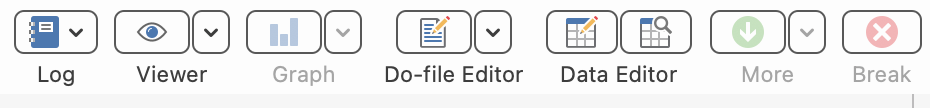
\includegraphics[keepaspectratio,alt={Stata Toolbar on OSX}]{week1_ribbon.png}}
\caption{Stata Toolbar on OSX}
\end{figure}

Once we click the do-file editor button or type in \emph{doedit}, a blank do file will appear.

\begin{figure}
\centering
\pandocbounded{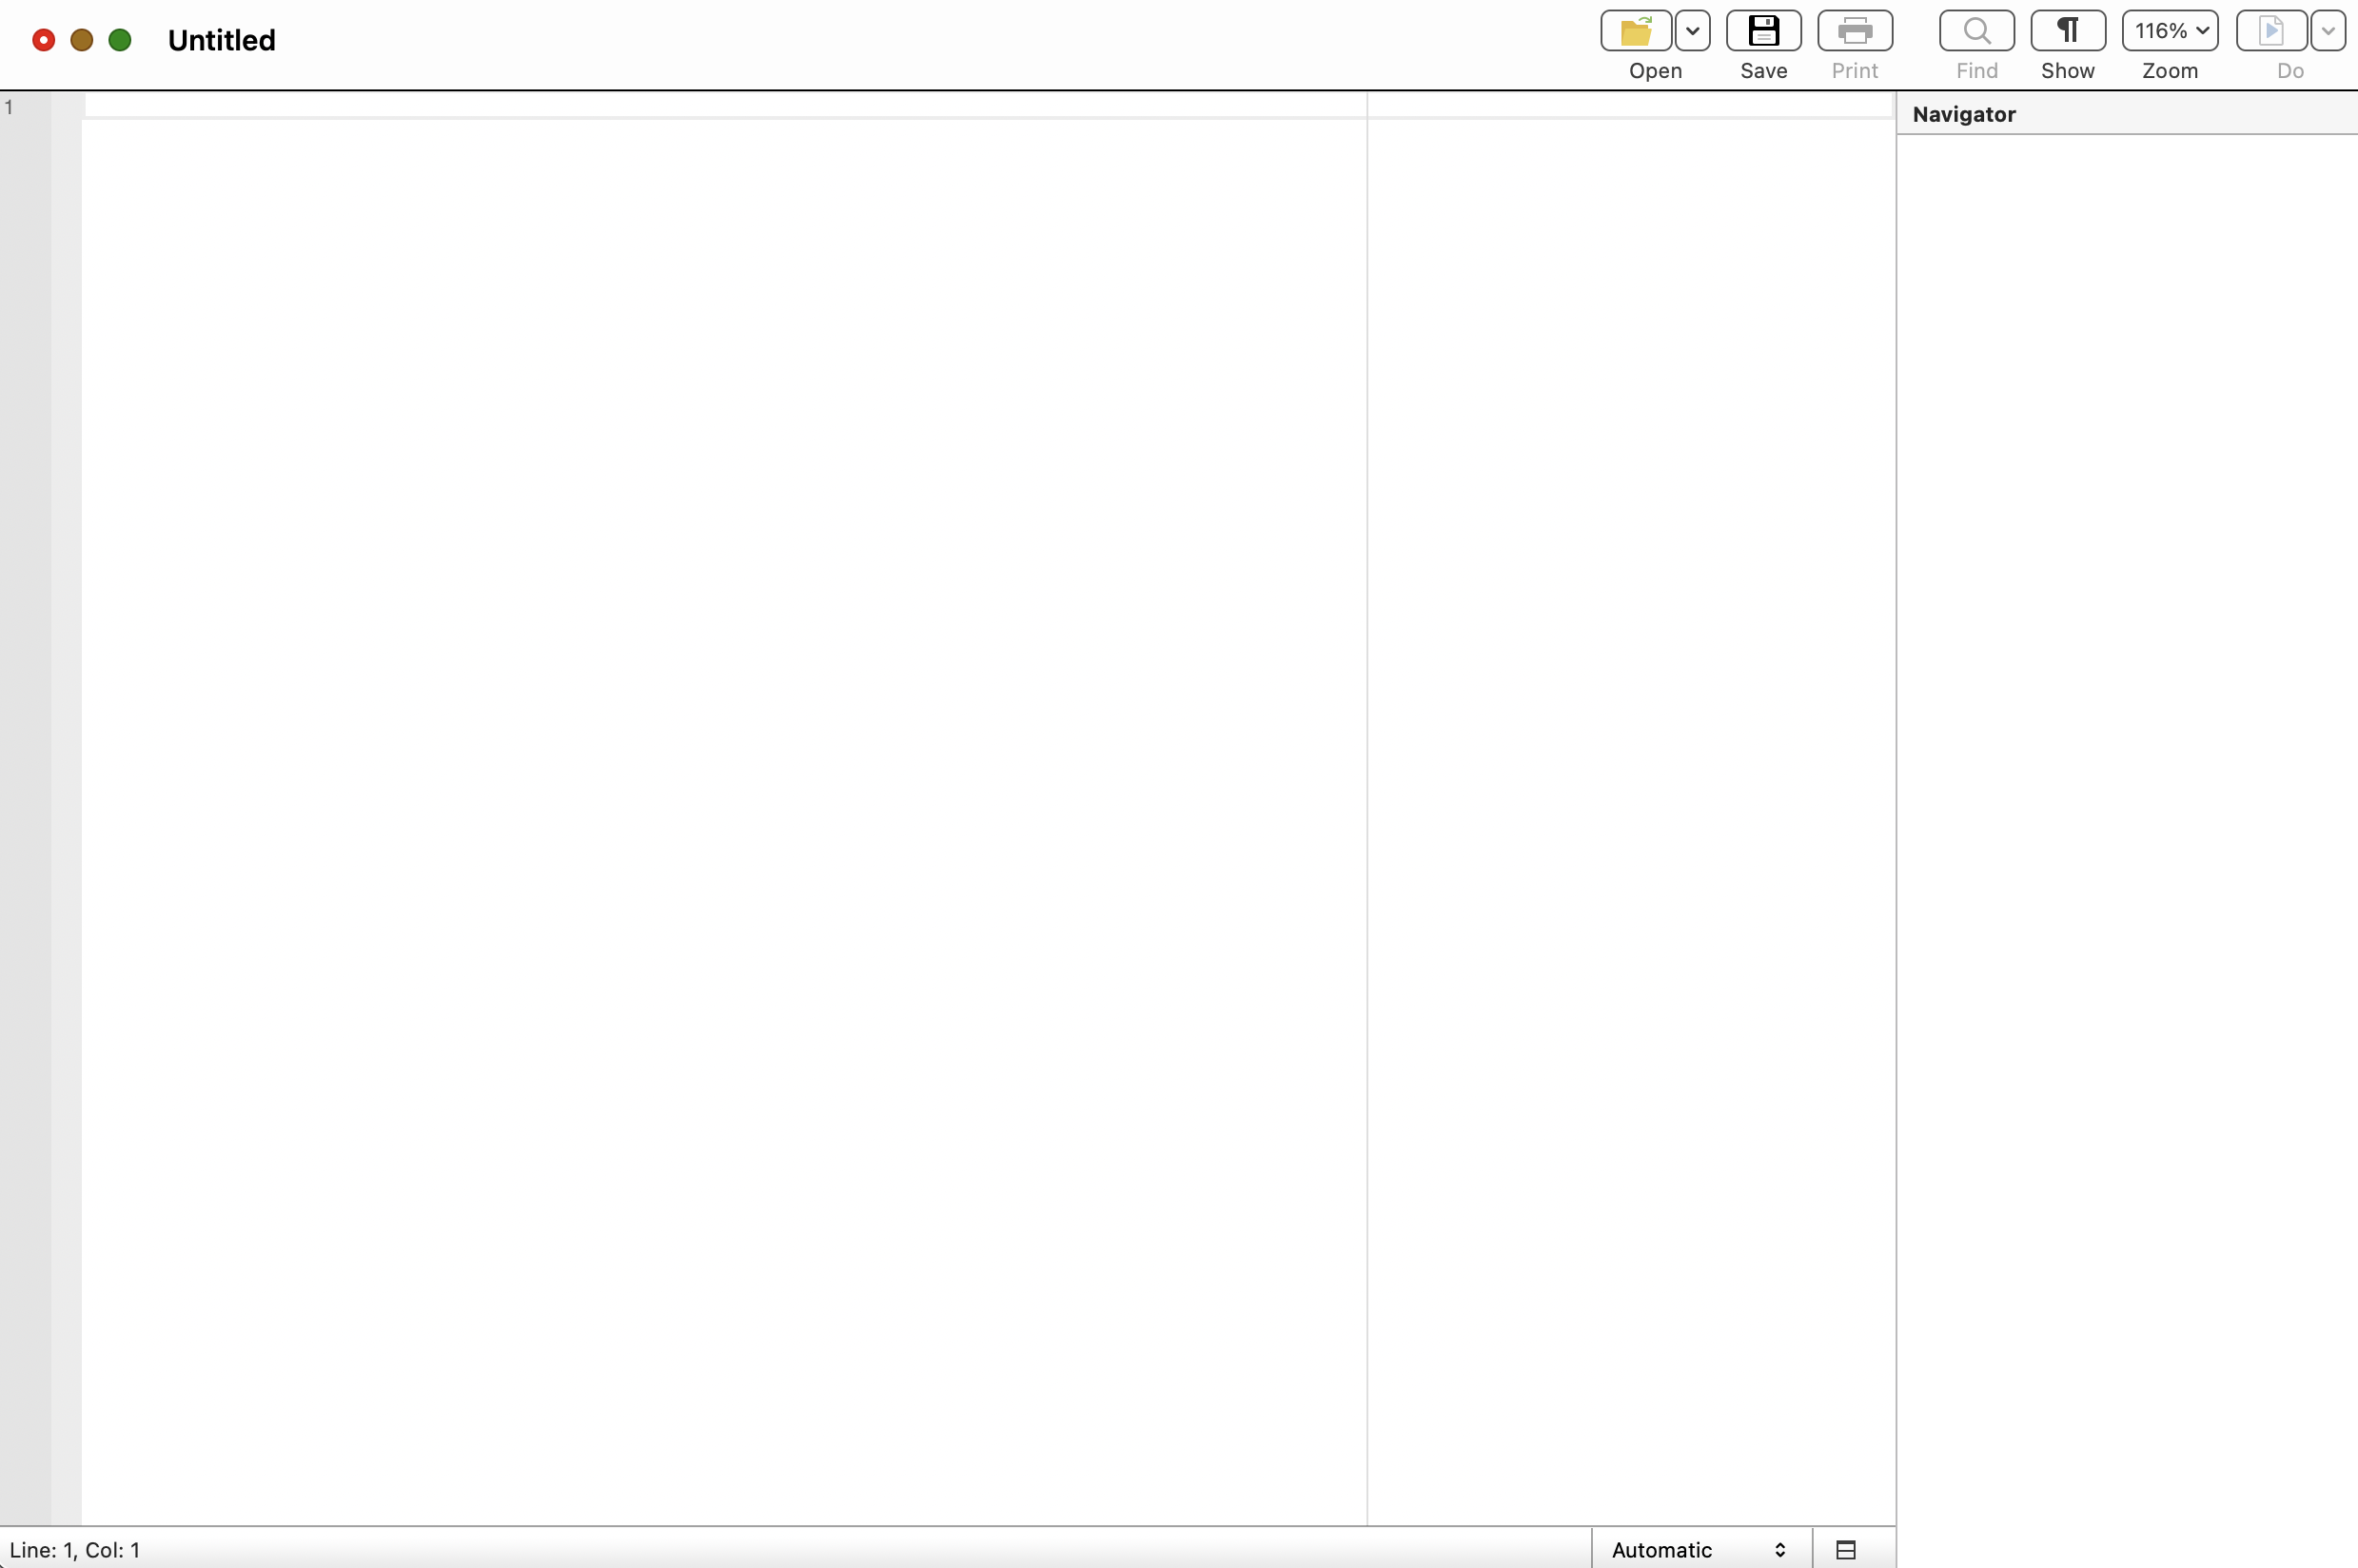
\includegraphics[keepaspectratio,alt={Blank Do File}]{week1_blankdo.png}}
\caption{Blank Do File}
\end{figure}

Let's go ahead and write our first do file.

It should look like this.
\pandocbounded{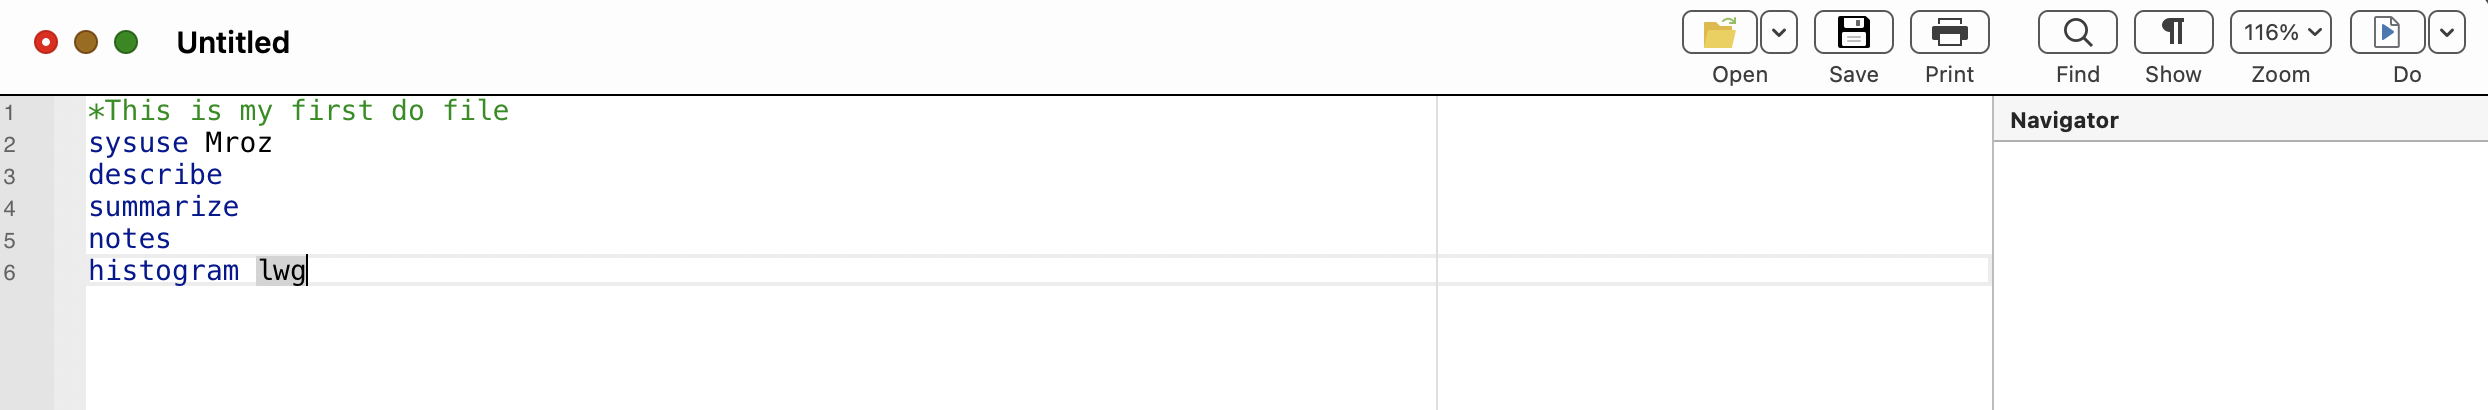
\includegraphics[keepaspectratio,alt={First Do File}]{week1_firstdo.png}}

Either click the ``Do'' button or press Ctrl+D for Windows or Shift+Command+D for OSX. Please note that you have some options with the do drop down menu.

\begin{Shaded}
\begin{Highlighting}[]
\NormalTok{*This is my first }\KeywordTok{do}\NormalTok{ file}
\KeywordTok{sysuse}\NormalTok{ Mroz}
\KeywordTok{describe}
\KeywordTok{summarize}
\KeywordTok{histogram}\NormalTok{ lwg}
\end{Highlighting}
\end{Shaded}

\begin{verbatim}
Contains data from /Users/Sam/Library/Application Support/Stata/ado/plus/M/Mroz.dt
> a
 Observations:           753                  
    Variables:             8                  2 May 2021 01:02
----------------------------------------------------------------------------------
Variable      Storage   Display    Value
    name         type    format    label      Variable label
----------------------------------------------------------------------------------
k5              byte    %8.0g                 Number of children 5 years old or
                                                younger
k618            byte    %8.0g                 Number of children 6 to 17 years old
age             byte    %8.0g                 Age in years
lwg             float   %9.0g                 Log wage rate. Actual wage, or for
                                                lfp=0 imputed by regressing lwg on
                                                other vars
inc             float   %9.0g                 Family income exclusive of wife\'s
                                                income
lfp             byte    %18.0g     lf         Labor-force participation
wc              byte    %27.0g     wcg        Wife attended college
hc              byte    %9.0g                 hcg
----------------------------------------------------------------------------------
Sorted by: 

    Variable |        Obs        Mean    Std. dev.       Min        Max
-------------+---------------------------------------------------------
          k5 |        753    .2377158     .523959          0          3
        k618 |        753    1.353254    1.319874          0          8
         age |        753    42.53785    8.072574         30         60
         lwg |        753    1.097115    .5875564  -2.054124   3.218876
         inc |        753    20.12897     11.6348      -.029         96
-------------+---------------------------------------------------------
         lfp |        753    .5683931    .4956295          0          1
          wc |        753    .2815405    .4500494          0          1
          hc |        753    .3917663    .4884694          0          1

(bin=27, start=-2.0541239, width=.19529629)
\end{verbatim}

\begin{figure}
\centering
\pandocbounded{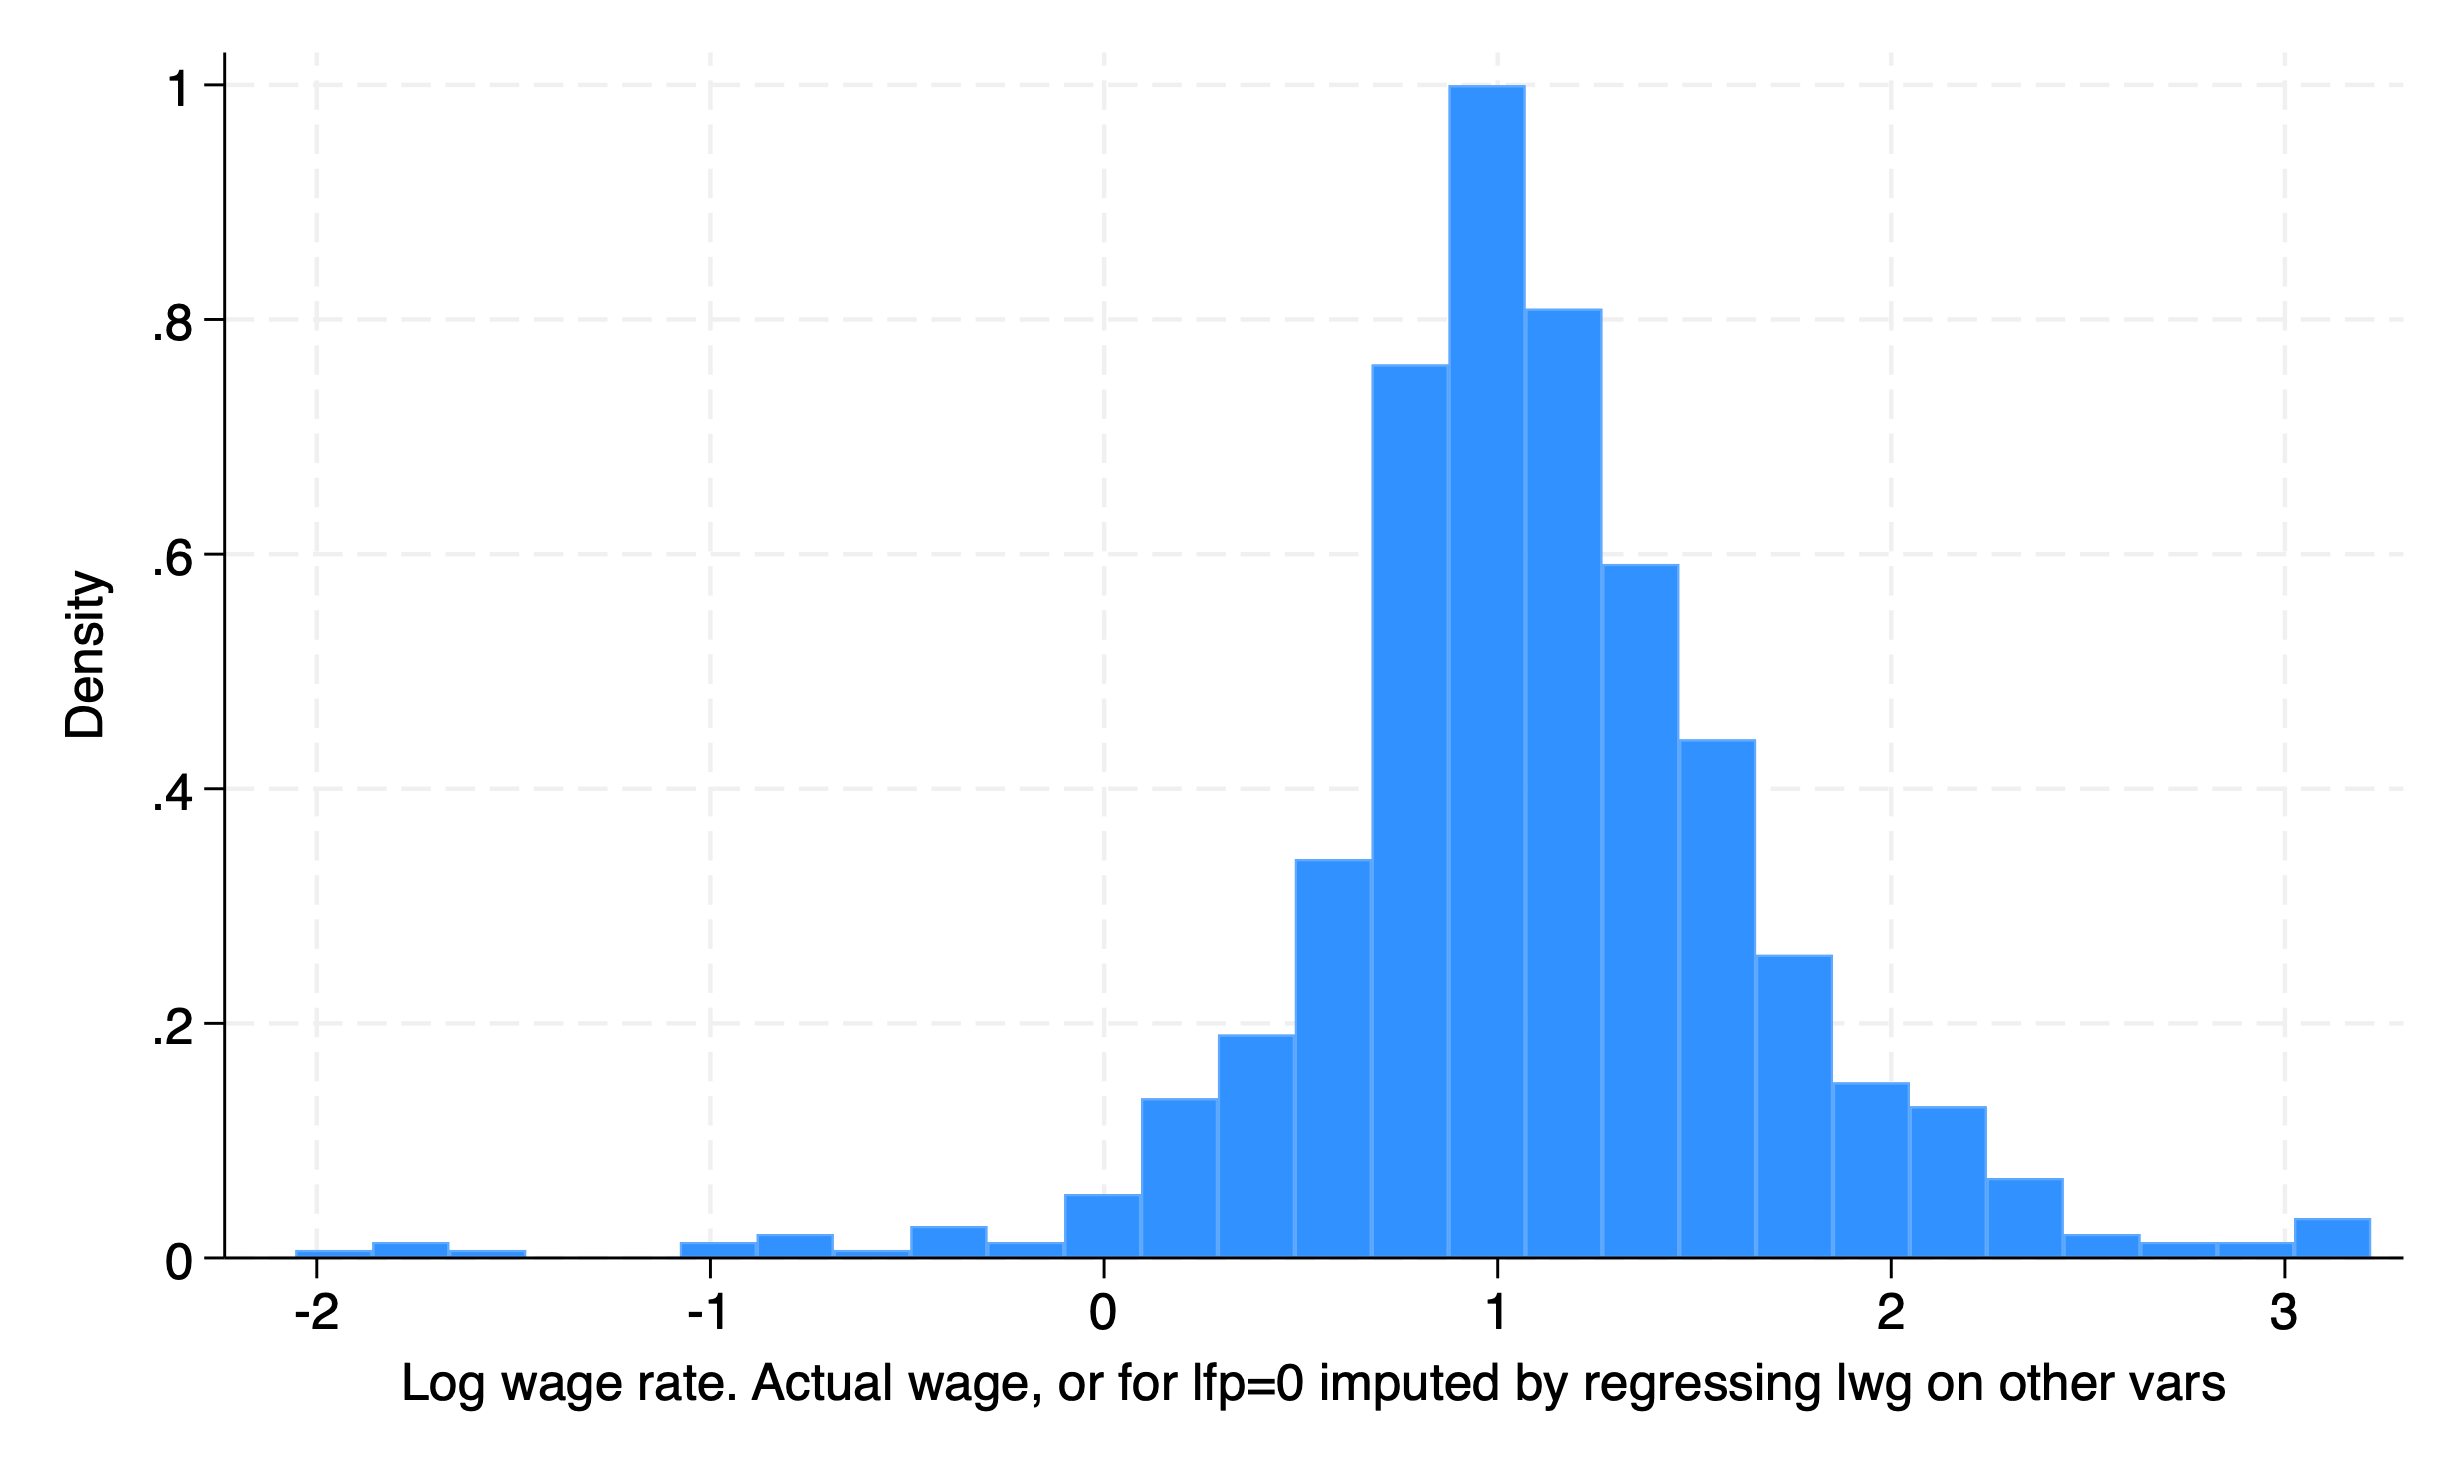
\includegraphics[keepaspectratio,alt={Histogram of natural log of wages from our first do file}]{week1_histlwg.png}}
\caption{Histogram of natural log of wages from our first do file}
\end{figure}

\section{Exporting Results}\label{exporting-results}

We'll start off with some very simple exporting of our results. We'll delve into better ETL tools later, but for now we will stick with the right-click copy-and-paste method.

Please note that I'm not a fan of the right-click copy-and-paste method, since it requires use input to complete. Acock (2020) provides a hint at some of Stata's tools for exporting results. This includes:

\begin{enumerate}
\def\labelenumi{\arabic{enumi}.}
\tightlist
\item
  \emph{esttab}
\item
  \emph{etable}
\item
  \emph{putexcel}
\item
  \emph{putdocx}
\item
  \emph{putpdf}
\item
  \emph{markdown}
\item
  \emph{dyndoc}
\end{enumerate}

Highlight your do file for all the rows except for the histogram. Click the drop down menu for the ``Do'' button and select ``execute selection''.

\begin{figure}
\centering
\pandocbounded{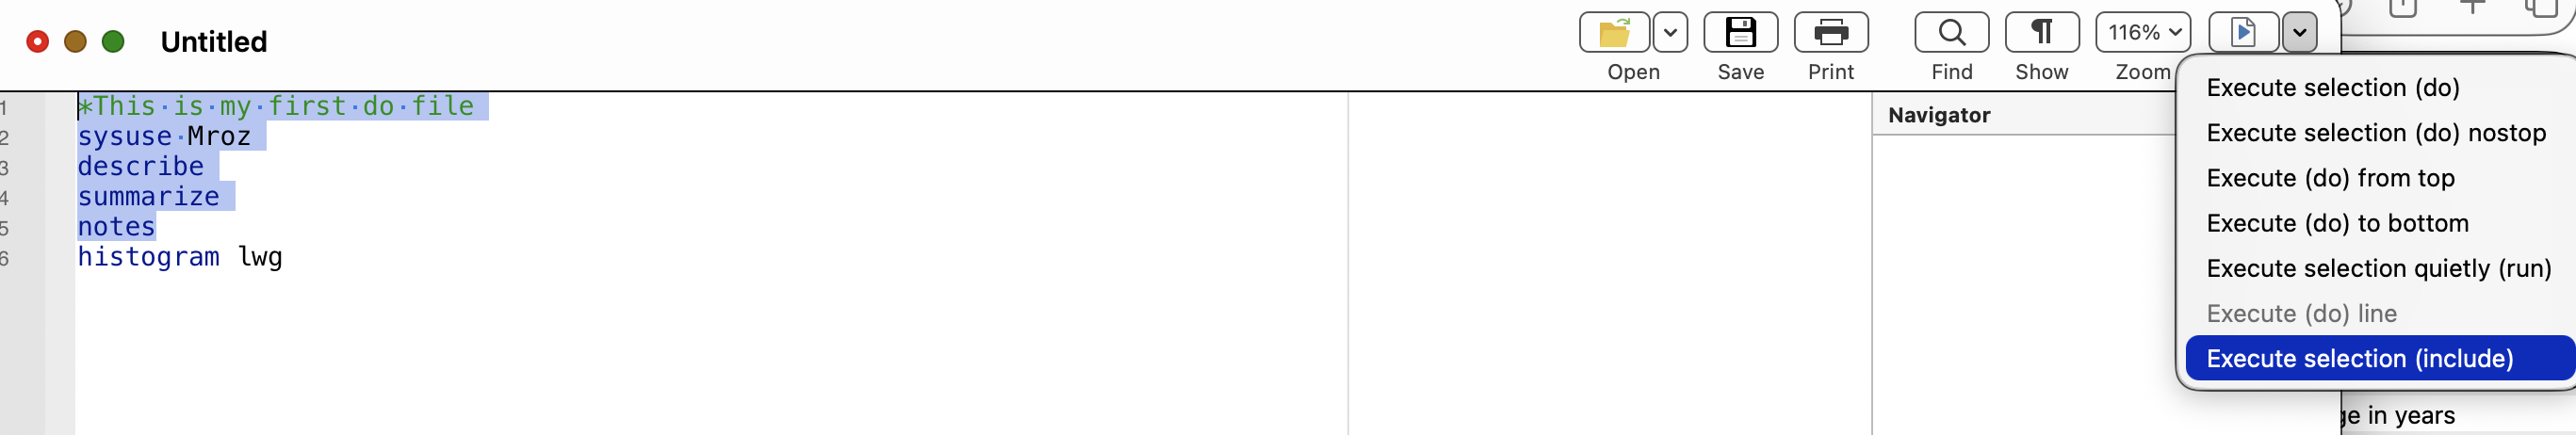
\includegraphics[keepaspectratio,alt={Highlight Do File}]{week1_selectdo.png}}
\caption{Highlight Do File}
\end{figure}

Now we have some output let's highlight the results and right click for options. Let's say we want to paste our table right into a Word document. We can select ``Copy as picture''. If we wanted to paste the results into an Excel file, we can select ``Copy as table''. If we wanted to paste right into a html file, we can select ``Copy as HTML''.

\begin{figure}
\centering
\pandocbounded{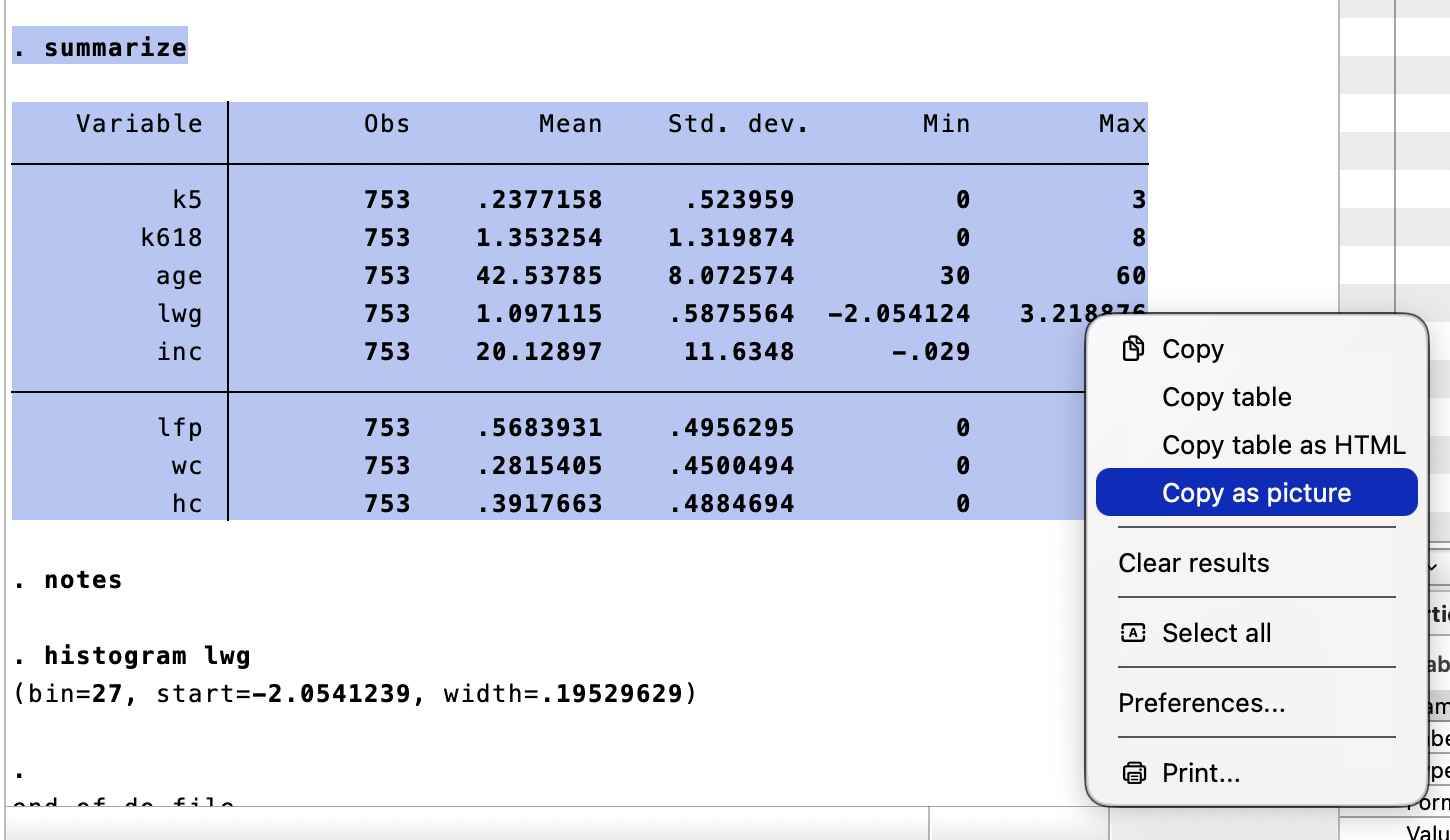
\includegraphics[keepaspectratio,alt={Highlight Results}]{week1_selectsum.png}}
\caption{Highlight Results}
\end{figure}

Now we can go to our Word document and paste it.

\begin{figure}
\centering
\pandocbounded{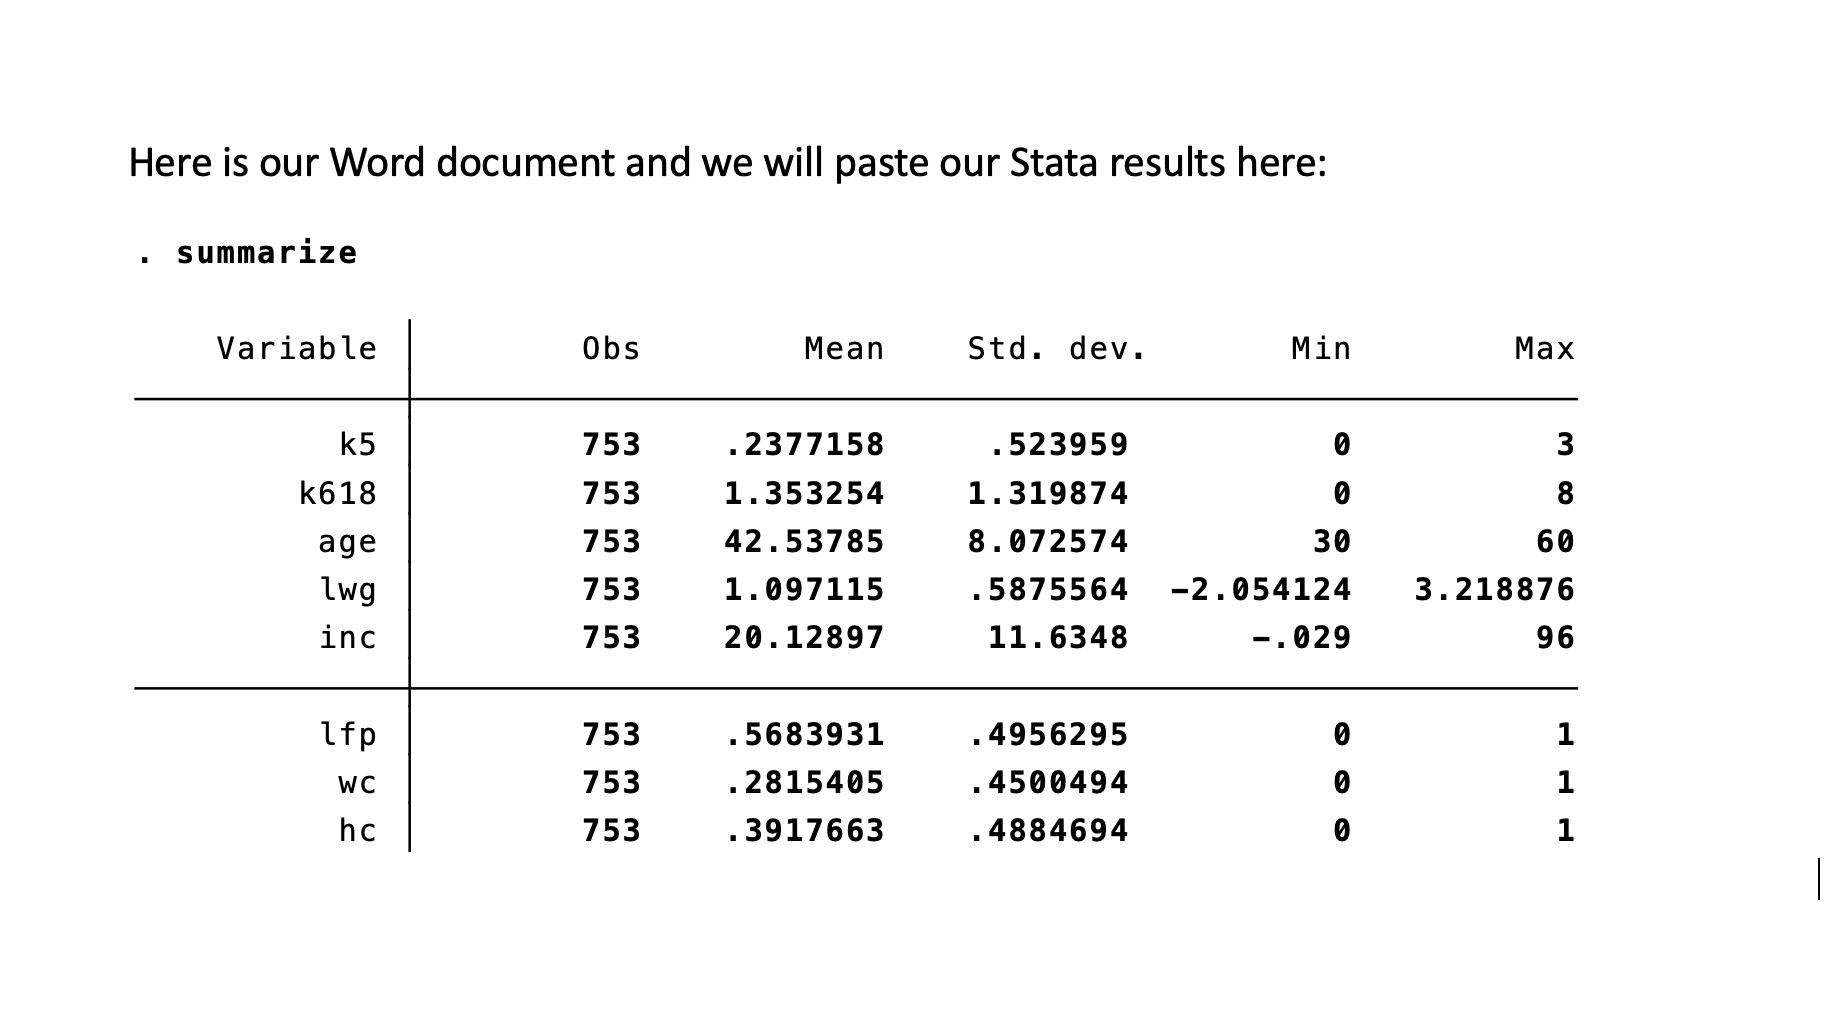
\includegraphics[keepaspectratio,alt={Paste our Stata results into Word}]{week1_worddoc.png}}
\caption{Paste our Stata results into Word}
\end{figure}

We can also export out in LaTex, which we will discuss next week with the LyX word processor. Another option is Overleaf for working with LaTex.

Or, we can utilize Stata with RMarkdown as you see here. These pages are built with the Bookdown package that utilizes RMarkdown with Stata being called.

\section{Logs}\label{logs}

We will cover log files a bit later in Mitchel (2020). But as a preview, you will need to use log files for your homework. However, I recommend not using log files until your syntax is working well. I have had plenty of do files fail to run since a log file was not properly closed during testing.

\chapter{References}\label{references}

Acock, A.C. (2023). A gentle introduction to Stata. 6th ed.~Stata Press

Mitchell, M. N. (2020). Data management using Stata: A practical handbook. Stata Press.

\bibliography{book.bib,packages.bib}

\end{document}
